%%%%%%%%%%%%%%%%%%%%%%%%%%%%%%%%%%%%%%%%%
% Beamer Presentation
% LaTeX Template
% Version 1.0 (10/11/12)
%
% This template has been downloaded from:
% http://www.LaTeXTemplates.com
%
% License:
% CC BY-NC-SA 3.0 (http://creativecommons.org/licenses/by-nc-sa/3.0/)
%
%%%%%%%%%%%%%%%%%%%%%%%%%%%%%%%%%%%%%%%%%

%----------------------------------------------------------------------------------------
%	PACKAGES AND THEMES
%----------------------------------------------------------------------------------------

\documentclass{beamer}

\mode<presentation> {

%\usetheme{default}
%\usetheme{AnnArbor}
%\usetheme{Antibes}
%\usetheme{Bergen}
%\usetheme{Berkeley}
%\usetheme{Berlin}
%\usetheme{Boadilla}
%\usetheme{CambridgeUS}
%\usetheme{Copenhagen}
%\usetheme{Darmstadt}
%\usetheme{Dresden}
%\usetheme{Frankfurt}
%\usetheme{Goettingen}
%\usetheme{Hannover}
%\usetheme{Ilmenau}
%\usetheme{JuanLesPins}
%\usetheme{Luebeck}
%\usetheme{Madrid}
%\usetheme{Malmoe}
%\usetheme{Marburg}
%\usetheme{Montpellier}
%\usetheme{PaloAlto}
\usetheme{Pittsburgh}
%\usetheme{Rochester}
%\usetheme{Singapore}
%\usetheme{Szeged}
%\usetheme{Warsaw}



%\usecolortheme{albatross}
\usecolortheme{beaver}
%\usecolortheme{beetle}
%\usecolortheme{crane}
%\usecolortheme{dolphin}
%\usecolortheme{dove}
%\usecolortheme{fly}
%\usecolortheme{lily}
%\usecolortheme{orchid}
%\usecolortheme{rose}
%\usecolortheme{seagull}
%\usecolortheme{seahorse}
%\usecolortheme{whale}
%\usecolortheme{wolverine}

%\setbeamertemplate{footline} % To remove the footer line in all slides uncomment this line
%\setbeamertemplate{footline}[page number] % To replace the footer line in all slides with a simple slide count uncomment this line

%\setbeamertemplate{navigation symbols}{} % To remove the navigation symbols from the bottom of all slides uncomment this line
}

\usepackage{graphicx} % Allows including images
\usepackage{booktabs} % Allows the use of \toprule, \midrule and \bottomrule in tables
%\usepackage{ctex}
\usepackage{multicol}
\usepackage{amsmath, amssymb, bm}
\usepackage{tikz}
\usetikzlibrary{positioning}
\usetikzlibrary{calc}
\usepackage[most]{tcolorbox}

\usepackage{fontspec}
\setsansfont{Calibri}[
    Path=Font/,
    Scale=0.9,
    Extension = .ttf,
    UprightFont=*-Regular,
    BoldFont=*-Bold,
    ItalicFont=*-Italic,
    BoldItalicFont=*-BoldItalic
    ]
\usepackage{unicode-math}

% \setmathfont{Libertinus Math} % 使用默认的数学字体或你偏好的数学字体 Latin Modern Math

\usepackage{ragged2e}
\justifying\let\raggedright\justifying %两端对齐

% Math operator shortcuts used throughout the deck
\newcommand{\E}{\mathbb{E}}
\newcommand{\Var}{\mathrm{Var}}
\newcommand{\Cov}{\mathrm{Cov}}
\newcommand{\tld}[1]{\widetilde{#1}}

\setbeamercolor{postit}{fg=black,bg=yellow!20}
\definecolor{postit}{rgb}{1,1,0.8} % xcolor name for tikz fill / tcolorbox colback

%--------
%	TITLE PAGE
%--------

\title[Asset Pricing]{\textbf{Asset Pricing}} % The short title appears at the bottom of every slide, the full title is only on the title page

\subtitle{Capstone: One Equation, Nine Lectures, and Beyond}

\author[Cheng Hang]{Cheng Hang} % Your name
\institute[DUFE] 
{School of Fintech \\
Dongbei University of Finance \& Economics \\ 
\medskip
\textbf{chenghangch@qq.com}
}
\date{\today} 

	\AtBeginSection[]
{
	\begin{frame}{Content}
		\small
		\begin{columns}[t]
		\begin{column}{0.5\textwidth}
		\tableofcontents[sections={1-6},sectionstyle=show/shaded,subsectionstyle=hide]
		\end{column}
		\begin{column}{0.5\textwidth}
		\tableofcontents[sections={7-12},sectionstyle=show/shaded,subsectionstyle=hide]
		\end{column}
		\end{columns}
		\addtocounter{framenumber}{-1}
	\end{frame}
}

%----------------------------------------------------------------------------------------
%	Begin
%----------------------------------------------------------------------------------------

\begin{document}

\begin{frame}
\titlepage % Print the title page as the first slide
\end{frame}

\section{Roadmap: One Equation Runs the Whole Course}

\begin{frame}{Welcome to the Last Class: What We Are Doing Today}
\begin{block}{The master claim of the whole course}
\centering\large All of asset pricing is one equation, $1 = \E_t[m\,R]$; \\[2pt]
\textbf{every model is just a different story about $m$.}
\end{block}
\justifying
This is a \alert{synthesis-and-outlook} capstone, not new material. We do three things:
\begin{itemize}
  \item \textbf{Recap} lectures 01--09 through \alert{one lens} -- the stochastic discount factor (SDF) $m$ -- so nine separate decks become a single journey.
  \item \textbf{Look outward} to five live research \textbf{frontiers}: a roughly \alert{60/40 split} between recap and outlook.
  \item Build not more facts but a \alert{mental map} -- where every model, puzzle, and fight sits on the same equation.
\end{itemize}
Everything organizes around \alert{two questions $m$ must answer} and \alert{three recurring tensions}:
\begin{itemize}
  \item \textbf{Time series:} why do discount rates / risk premia \textit{vary over time}?
  \item \textbf{Cross-section:} why do \textit{average returns differ} across assets?
  \item Tensions: \textcolor{red}{risk vs.\ behavioral} \ $\bullet$\ \textcolor{red}{structural vs.\ reduced-form} \ $\bullet$\ \textcolor{red}{US vs.\ China}.
\end{itemize}
\end{frame}

\begin{frame}{The Course as One Journey}
\centering
\resizebox{\textwidth}{!}{%
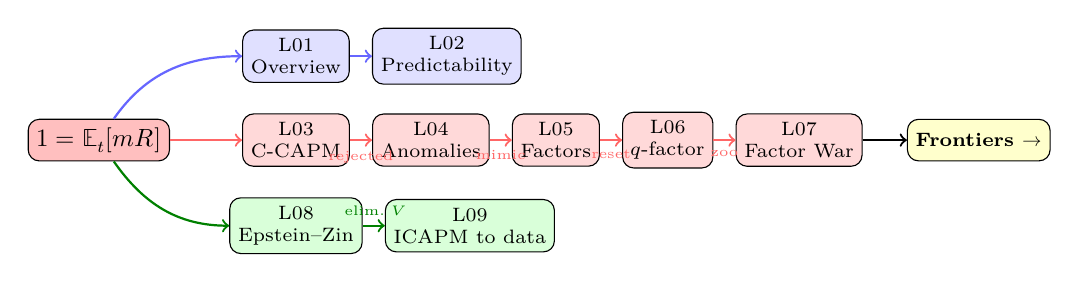
\begin{tikzpicture}[
  box/.style={draw,rounded corners,align=center,inner sep=3pt,minimum height=15pt,font=\scriptsize},
  ts/.style={box,fill=blue!12},
  cs/.style={box,fill=red!15},
  st/.style={box,fill=green!15},
  hub/.style={box,fill=red!25,font=\small\bfseries}]

  % Cross-section spine (the long one) -- anchors the layout
  \node[cs] (l3) {L03\\C-CAPM};
  \node[cs, right=8pt of l3] (l4) {L04\\Anomalies};
  \node[cs, right=8pt of l4] (l5) {L05\\Factors};
  \node[cs, right=8pt of l5] (l6) {L06\\$q$-factor};
  \node[cs, right=8pt of l6] (l7) {L07\\Factor War};

  % Time-series spine (above) and structural spine (below)
  \node[ts, above=11pt of l3] (l1) {L01\\Overview};
  \node[ts, right=8pt of l1] (l2) {L02\\Predictability};
  \node[st, below=11pt of l3] (l8) {L08\\Epstein--Zin};
  \node[st, right=8pt of l8] (l9) {L09\\ICAPM to data};

  % The hub on the left; frontiers on the right
  \node[hub, left=26pt of l3] (eq) {$1=\E_t[m R]$};
  \node[box,fill=postit, right=16pt of l7, font=\scriptsize\bfseries] (fr) {Frontiers $\to$};

  \draw[thick,->,blue!60] (eq) to[out=55,in=180] (l1);
  \draw[thick,->,blue!60] (l1) -- (l2);
  \draw[thick,->,red!60] (eq) -- (l3);
  \draw[thick,->,red!60] (l3) -- node[below,font=\tiny]{rejected} (l4);
  \draw[thick,->,red!60] (l4) -- node[below,font=\tiny]{mimic} (l5);
  \draw[thick,->,red!60] (l5) -- node[below,font=\tiny]{reset} (l6);
  \draw[thick,->,red!60] (l6) -- node[below,font=\tiny]{zoo} (l7);
  \draw[thick,->,green!50!black] (eq) to[out=-55,in=180] (l8);
  \draw[thick,->,green!50!black] (l8) -- node[above,font=\tiny]{elim.\ $V$} (l9);
  \draw[thick,->] (l7) -- (fr);
\end{tikzpicture}}

\vspace{2pt}
\footnotesize
\textcolor{blue}{$\blacksquare$ Time series} \quad
\textcolor{red}{$\blacksquare$ Cross-section} \quad
\textcolor{green!50!black}{$\blacksquare$ Structural theory}
\par\smallskip
\justifying One equation at the top; three spines hang off it; every edge is a \alert{logical move} (CAPM rejected $\to$ anomalies; empirical patch vs.\ structural reset $\to$ q-factor; eliminate the continuation value $\to$ two-beta ICAPM). All roads then point right, to the frontiers.
\end{frame}

\begin{frame}{The One Equation: $1 = \E_t[m\,R]$}
\justifying
Start from the only equation we never abandon:
\begin{align}
  1 &= \E_t\!\left[m_{t+1}\,R_{t+1}\right] \\[2pt]
  \Longleftrightarrow\quad P_t &= \E_t\!\left[m_{t+1}\cdot \text{payoff}_{t+1}\right].
\end{align}
\begin{itemize}
  \item \textbf{Price = expected discounted payoff.} Today's price is the expected, $m$-weighted future payoff -- cash flows \textit{and} discount rates folded into one object.
  \item $m_{t+1}$ is a \alert{single random variable} that must price \textbf{all} assets at once: stocks, bonds, options, FX -- the whole cross-section, simultaneously.
  \item $m$ is \alert{unobservable}. So asset pricing is a scientific \textit{search for $m$}, the way physicists search for a law \href{https://doi.org/10.1111/j.1540-6261.2011.01671.x}{\textcolor{blue}{(Cochrane 2011)}}.
\end{itemize}
\begin{block}{The joint-hypothesis problem}
When a candidate SDF fails to price assets, we cannot tell \textit{why}: the market may be \textcolor{red}{inefficient}, \textbf{or} our $m$ may simply be \textcolor{red}{wrong}. The two can never be cleanly separated -- a tension that haunts every empirical test ahead.
\end{block}
\end{frame}

\begin{frame}{Every Model Is a Story About $m$}
\justifying
The whole course is one equation read nine ways -- each lecture proposes a different $m$:
\begin{center}\footnotesize
\begin{tabular}{@{}ll@{}}
\toprule
\textbf{Model (lecture)} & \textbf{Story about $m$} \\
\midrule
C-CAPM (L03) & $m=\beta\!\left(C_{t+1}/C_t\right)^{-\gamma}$ \\
CAPM (L03) & $m = a + b\,R^{W}$ \\
FF / multifactor (L05) & $m = a + b'f$,\; $f=$ MKT, SMB, HML, $\dots$ \\
q-factor (L06) & $m$ disciplined by firm investment FOC \\
Epstein--Zin (L08) & $m=\delta\!\left(\tfrac{C'}{C}\right)^{-1/\psi}\!\!\left(\tfrac{V'}{\mu(V)}\right)^{-(\gamma-1/\psi)}$ \\
ICAPM, Campbell (L09) & $\tld{m}=-\gamma\,\tld{r}_w-(\gamma-1)\,\tld{h}$ \\
\bottomrule
\end{tabular}
\end{center}
\smallskip
\begin{itemize}
  \item \textbf{Different stories, one equation.} From consumption MRS, to the market return, to linear factors, to the firm's investment margin, to recursive preferences.
  \item Every story is judged on the \alert{same two questions}: can its $m$ make \textcolor{blue}{discount rates vary over time}, and can it explain \textcolor{red}{why average returns differ in the cross-section}?
\end{itemize}
\end{frame}

\section{The SDF and Its Equivalent Faces}

\begin{frame}{From Euler Equation to the SDF (Step 1)}
\small
The investor chooses how much of asset $i$ (price $p_t$, payoff $x_{t+1}$) to buy, solving
\begin{equation*}
\max_{\{\xi\}}\ \E_t\!\left[\sum_{s=0}^{\infty}\beta^{s}\, u(C_{t+s})\right]
\quad\text{s.t.}\quad C_t = e_t - p_t\,\xi,\ \ C_{t+1}=e_{t+1}+x_{t+1}\,\xi .
\end{equation*}
\textbf{First-order condition} (derivative in the quantity $\xi$, one step at a time):
\begin{align*}
0 &= -\,p_t\, u'(C_t) + \E_t\!\big[\beta\, u'(C_{t+1})\, x_{t+1}\big],\\
p_t\, u'(C_t) &= \E_t\!\big[\beta\, u'(C_{t+1})\, x_{t+1}\big],\\
p_t &= \E_t\!\left[\beta\,\frac{u'(C_{t+1})}{u'(C_t)}\,x_{t+1}\right].
\end{align*}
\begin{block}{Define the stochastic discount factor}
\[
M_{t+1} \equiv \beta\,\frac{u'(C_{t+1})}{u'(C_t)}
\quad\Longrightarrow\quad
\boxed{\,p_t=\E_t[M_{t+1}\,x_{t+1}]\,},\qquad \boxed{\,1=\E_t[M_{t+1}R_{t+1}]\,}.
\]
\end{block}
\alert{The \emph{form} $1=\E_t(MR)$ is preference-free; every model is just a different \textit{story} about $M$.}\hfill {\scriptsize(foundation: L03)}
\end{frame}

\begin{frame}{Face 1 --- Risk Premium as $-\Cov(R,m)$ (Step 2)}
\small
Start from $1=\E_t[m\,R^i]$ and use the covariance identity $\E(mR)=\E(m)\E(R)+\Cov(m,R)$:
\begin{align*}
1 &= \E_t(m)\,\E_t(R^i) + \Cov_t(m,R^i).
\end{align*}
The risk-free asset has a certain return, so $\Cov_t(m,R_f)=0$ and
\[
1=\E_t(m)\,R_f \quad\Longrightarrow\quad \E_t(m)=\tfrac{1}{R_f}.
\]
Substitute and rearrange for the \textbf{excess return}:
\begin{align*}
1 &= \tfrac{1}{R_f}\,\E_t(R^i) + \Cov_t(m,R^i),\\
\E_t(R^i) &= R_f - R_f\,\Cov_t(m,R^i),\\
\boxed{\ \E_t(R^i)-R_f = -\,R_f\,\Cov_t(m,R^i)\ }.
\end{align*}
In logs (Jensen term $\sigma_i^2/2$): $\quad\E_t[r_i-r_f]+\tfrac{\sigma_i^2}{2}=-\,\sigma_{im}.$
\begin{block}{The conceptual heart}
Only \alert{covariance with $m$} is priced. An asset that pays off when $m$ is high (bad times, high marginal utility) is \textbf{insurance} $\Rightarrow$ low / negative premium. Idiosyncratic risk uncorrelated with $m$ earns \textbf{nothing}.
\end{block}
\end{frame}

\begin{frame}{Face 2 --- Beta Pricing: the SDF \emph{is} a Factor Model (Step 3)}
\small
Project $m$ onto the space of payoffs $X$: $\ m = x^{*} + \varepsilon$ with $x^{*}=\mathrm{proj}(m\mid X)$ and $\E(\varepsilon\,X)=0$. Since $\varepsilon$ is orthogonal to all returns, $x^{*}$ prices everything. Rewriting Face 1:
\begin{align*}
\E_t(R^i)-R_f &= -\,R_f\,\Cov_t(m,R^i)\\
&= \underbrace{\frac{\Cov_t(R^i,m)}{\Var_t(m)}}_{\textstyle \beta_{i,m}}\cdot\underbrace{\Big(-R_f\,\Var_t(m)\Big)}_{\textstyle \lambda_m}\\
&= \beta_{i,m}\,\lambda_m .
\end{align*}
If $m$ is \textbf{linear in factors}, $m=a+b'f$, the same algebra gives the multifactor form
\[
\boxed{\ \E_t(R^i)-R_f=\beta_i'\,\lambda\ },\qquad \beta_i=\Var(f)^{-1}\Cov(f,R^i).
\]
\textbf{CAPM} is the special case $m=a+b\,R^{W}$ (quadratic utility / market efficiency).
\begin{block}{Punchline (revisited in Frontier I)}
$1=\E(mR)$ and expected-return--beta pricing are \alert{mathematically equivalent representations of the same object}: ``estimate $m$'' $=$ ``find the factors.''
\end{block}
\end{frame}

\begin{frame}{Face 3 --- MV Frontier \& the Hansen--Jagannathan Bound (Step 4)}
\small
From Face 1, $\E(R^{e})=-R_f\,\Cov(m,R^{e})=-R_f\,\rho_{m,R^e}\,\sigma(m)\,\sigma(R^{e})$ for any excess return $R^{e}$. Rearranging and using $\big|\rho_{m,R^e}\big|\le 1$:
\begin{align*}
\frac{\big|\E(R^{e})\big|}{\sigma(R^{e})}
&= R_f\,\big|\rho_{m,R^e}\big|\,\sigma(m)
\ \le\ R_f\,\sigma(m)
= \frac{\sigma(m)}{\E(m)} .
\end{align*}
Maximizing the left side over all assets gives the \textbf{Hansen--Jagannathan bound}:
\[
\boxed{\ \frac{\sigma(m)}{\E(m)}\ \ge\ \max_{R^e}\ \frac{\big|\E(R^{e})\big|}{\sigma(R^{e})}=\max\ \text{Sharpe ratio}\ }.
\]
The bound is \alert{tight} ($\rho_{m,R^e}=-1$) exactly at the \textbf{tangency / MV-efficient} portfolio: there the SDF is spanned by (is a linear function of) the maximum-Sharpe portfolio.
\begin{block}{Two puzzles this seeds}
\begin{itemize}\itemsep1pt
\item \textbf{Equity-premium puzzle:} a $\sim$0.5 market Sharpe forces $\sigma(m)/\E(m)$ huge, hence implausible risk aversion (\href{https://doi.org/10.1016/0304-3932(85)90061-3}{\textcolor{blue}{Mehra--Prescott (1985)}}).
\item \textbf{Factor-war criterion (L07):} the best model is the one whose factors attain the max squared Sharpe ratio (\href{https://doi.org/10.1016/j.jfineco.2018.02.012}{\textcolor{blue}{Fama--French (2018)}}).
\end{itemize}
\end{block}
\end{frame}

\begin{frame}{Face 4 --- Risk-Neutral Pricing (Step 5)}
\small
Use $m$ to bend the probabilities. With $\E_t(m)=1/R_f$, define the \textbf{risk-neutral measure} $\mathbb{P}^{*}$ by the change of measure
\[
\frac{d\mathbb{P}^{*}}{d\mathbb{P}} \equiv \frac{m_{t+1}}{\E_t(m_{t+1})} = R_f\, m_{t+1}\ \ (\ge 0,\ \E_t=1).
\]
Then any price becomes a \emph{risk-free-discounted} expectation under $\mathbb{P}^{*}$:
\begin{align*}
p_t &= \E_t(m\,x) = \E_t(m)\,\E^{*}_t(x) = \frac{1}{R_f}\,\E^{*}_t(x_{t+1}),
\end{align*}
where $\E^{*}_t[\cdot]=\E_t\!\big[(R_f m)\,\cdot\big]$. \alert{All risk corrections are pushed into the probabilities}; discounting is at the riskless rate.
\begin{block}{One object, four faces}
\centering
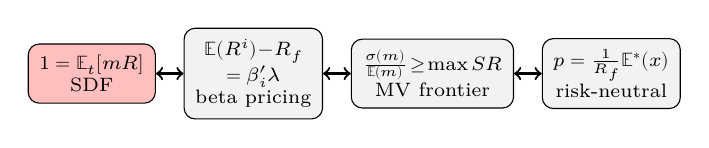
\begin{tikzpicture}[box/.style={draw,rounded corners,align=center,inner sep=4pt,minimum height=20pt,font=\scriptsize},
stage/.style={box,fill=gray!10}, here/.style={box,fill=red!25}]
\node[here] (sdf) {$1=\E_t[m R]$\\SDF};
\node[stage,right=10pt of sdf] (beta) {$\E(R^i)\!-\!R_f$\\$=\beta_i'\lambda$\\beta pricing};
\node[stage,right=10pt of beta] (mv) {$\frac{\sigma(m)}{\E(m)}\!\ge\!\max SR$\\MV frontier};
\node[stage,right=10pt of mv] (rn) {$p=\frac1{R_f}\E^{*}(x)$\\risk-neutral};
\draw[<->,thick] (sdf)--(beta); \draw[<->,thick] (beta)--(mv); \draw[<->,thick] (mv)--(rn);
\end{tikzpicture}
\end{block}
\centering\textbf{SDF $\equiv$ beta pricing $\equiv$ MV frontier $\equiv$ risk-neutral measure.} This equivalence is \emph{why the whole course is one equation}.
\end{frame}

\section{The Time-Series Question: Why Discount Rates Vary}

\begin{frame}{Reframing the Question: Predictability $=$ Time-Varying $m$}
We have re-derived the master equation $1 = \E_t[m_{t+1}R_{t+1}]$. Now ask the \alert{first organizing question}: why do conditional expected returns -- discount rates -- move over \textit{time}?

\begin{itemize}
  \item The empirical test is a single \textbf{predictive regression} (L02):
  \begin{equation*}
    R_{t+1} = a + b\,x_t + \varepsilon_{t+1}.
  \end{equation*}
  \item $b \neq 0$ means $\E_t[R_{t+1}]$ -- the risk premium, the discount rate -- \alert{varies with the state} $x_t$. A nonzero $b$ or large $R^2$ is the empirical face of a \textbf{time-varying SDF}.
  \item The efficient-markets benchmark $b=0,\ R^2=0$ is a \textbf{theory} (constant $m$), \textit{not} a fact. ``Returns are unpredictable'' is a maintained hypothesis.
  \item Tie to the kernel: a time-varying $m$ generates a time-varying conditional $\E_t[R]$. The two are the same statement.
\end{itemize}

\begin{block}{The organizing claim}
\href{https://doi.org/10.1111/j.1540-6261.2011.01671.x}{\textcolor{blue}{Cochrane (2011)}}, ``Discount Rates'': \textit{discount-rate variation} is the central time-series question of modern asset pricing. ``Predictable'' means conditional-mean variation, not perfect forecastability.
\end{block}
\end{frame}

\begin{frame}{The Campbell--Shiller Identity (Step-by-Step)}
\small
Predictability is not a model -- it is an \alert{accounting identity}. Start from the loglinearized one-period return ($\rho \approx 0.96$ annual):
\begin{align*}
  r_{t+1} &\approx k + \rho\,p_{t+1} + (1-\rho)\,d_{t+1} - p_t \\[2pt]
  \text{rearrange to put } p_t-d_t \text{ on the left:}\quad
  p_t - d_t &\approx -k + \rho\,(p_{t+1}-d_{t+1}) + (d_{t+1}-d_t) - r_{t+1}\\[2pt]
  \text{i.e. } \quad d_t - p_t &\approx -k - \rho\,(d_{t+1}-p_{t+1}) + r_{t+1} - \Delta d_{t+1}.
\end{align*}
Iterate forward, imposing $\lim_{j\to\infty}\rho^{\,j}(d_{t+j}-p_{t+j})=0$:
\begin{equation*}
  \boxed{\;d_t - p_t \approx -\frac{k}{1-\rho} + \sum_{j=0}^{\infty}\rho^{\,j}\bigl[\,r_{t+1+j} - \Delta d_{t+1+j}\,\bigr]\;}
\end{equation*}
\begin{itemize}
  \item A \textbf{high $d-p$ MUST forecast} high future returns and/or low future dividend growth. There is no third possibility -- it is algebra, not behavior.
  \item Confirmed empirically: \href{https://doi.org/10.1016/0304-405X(88)90020-7}{\textcolor{blue}{Fama--French (1988)}}, \href{https://doi.org/10.1016/0304-405X(89)90095-0}{\textcolor{blue}{Fama--French (1989)}}; defended in \href{https://doi.org/10.1093/rfs/hhm046}{\textcolor{blue}{Cochrane (2008)}}.
\end{itemize}
\end{frame}

\begin{frame}{Cash-Flow News vs.\ Discount-Rate News}
\small
Subtract the conditional expectation from the loglinear return: the \textit{innovation} splits mechanically into two pieces.
\begin{align*}
  (\E_{t+1}-\E_t)\,r_{t+1}
  &= \underbrace{(\E_{t+1}-\E_t)\sum_{j=0}^{\infty}\rho^{\,j}\Delta d_{t+1+j}}_{N_{CF,\,t}\;:\;\text{cash-flow news}} \\
  &\quad - \underbrace{(\E_{t+1}-\E_t)\sum_{j=1}^{\infty}\rho^{\,j} r_{t+1+j}}_{N_{DR,\,t}\;:\;\text{discount-rate news}} \\
  \Longrightarrow\quad (\E_{t+1}-\E_t)\,r_{t+1} &= N_{CF,\,t} - N_{DR,\,t}.
\end{align*}
\begin{itemize}
  \item \textbf{Higher discount rates} $\Rightarrow N_{DR}>0 \Rightarrow$ \alert{capital loss}: same cash flows, discounted harder.
  \item An identity, not behavior -- agnostic between risk and mispricing; firm-level book-to-market version: \href{https://doi.org/10.1111/1540-6261.00437}{\textcolor{blue}{Vuolteenaho (2002)}}.
  \item \alert{The hinge into the cross-section}: $N_{DR}$ is itself a state variable, the priced ICAPM hedging factor of L08--L09.
\end{itemize}
\end{frame}

\begin{frame}{The Risk--Return Tradeoff and Why It ``Fails''}
\small
The conditional equity premium \textit{is} the ICAPM risk--return relation. \href{https://doi.org/10.2307/1913811}{\textcolor{blue}{Merton (1973)}}:
\begin{equation*}
  \E_t[R_{m,t+1}] = \mu + \gamma\,\sigma_t^2,
  \qquad\text{complete ICAPM:}\quad
  \E_t[R_{m,t+1}] = \gamma\,\sigma_{m,t}^2 + \lambda\,\sigma_{mf,t}.
\end{equation*}
Run the \textit{simple} regression of returns on variance, omitting the hedge term $\lambda\,\sigma_{mf}$:
\begin{align*}
  \text{plim }\hat\gamma
  &= \gamma + \lambda\,\frac{\Cov(\sigma_{m,t}^2,\ \sigma_{mf,t})}{\Var(\sigma_{m,t}^2)}
  \qquad\text{(Guo--Whitelaw OVB).}
\end{align*}
\begin{itemize}
  \item If $\lambda>0$ and variance co-moves \alert{negatively} with the hedge component, $\hat\gamma$ is biased down -- even \textbf{negative}. This is the empirical ``risk--return puzzle'' (\href{https://doi.org/10.1016/0304-405X(87)90045-6}{\textcolor{blue}{Campbell 1987}}; \href{https://doi.org/10.1111/j.1540-6261.1993.tb05128.x}{\textcolor{blue}{Glosten--Jagannathan--Runkle 1993}}).
  \item The relation is \textbf{restored} once the omitted state variable is included -- $cay$ (\href{https://doi.org/10.1111/j.1540-6261.2006.00877.x}{\textcolor{blue}{Guo--Whitelaw 2006}}) or idiosyncratic volatility (\href{https://doi.org/10.1016/j.jfineco.2005.10.003}{\textcolor{blue}{Guo--Savickas 2006}}), with plausible RRA $\approx 5$--$6$.
  \item \alert{Lesson}: the ``failure'' is omitted-variable bias, not a failure of risk-based theory.
\end{itemize}
\end{frame}

\begin{frame}{The Predictor Zoo and the Macro Predictors That Survive}
\small
A large ``zoo'' of time-series predictors exists; the credible ones are \alert{economically motivated} business-condition variables, not data-mined regressors.
\begin{itemize}
  \item \textbf{Valuation \& business-cycle (risk-motivated):}
  \begin{itemize}\small
    \item D/P, TERM, DEF -- countercyclical, common across stocks and bonds (\href{https://doi.org/10.1016/0304-405X(89)90095-0}{\textcolor{blue}{Fama--French 1989}}).
    \item $cay$, the consumption--wealth ratio (\href{https://doi.org/10.1111/0022-1082.00347}{\textcolor{blue}{Lettau--Ludvigson 2001}}).
    \item Output gap, a price-free production-based variable (\href{https://doi.org/10.1093/rfs/hhn087}{\textcolor{blue}{Cooper--Priestley 2009}}).
  \end{itemize}
  \item \textbf{Forward-looking / market-implied:}
  \begin{itemize}\small
    \item Variance risk premium (\href{https://doi.org/10.1093/rfs/hhp008}{\textcolor{blue}{Bollerslev--Tauchen--Zhou 2009}}).
    \item IPO first-day return as an ex-ante premium proxy (\href{https://doi.org/10.1093/rfs/hhr093}{\textcolor{blue}{Guo 2011}}).
    \item SVIX option-implied lower bound, no regression needed (\href{https://doi.org/10.1093/qje/qjw034}{\textcolor{blue}{Martin 2017}}).
  \end{itemize}
\end{itemize}
\begin{block}{China A-share angle}
The valuation ratio (pd) predicts returns \alert{negatively} and \alert{more strongly at long horizons} -- significant from roughly 9 months out -- an out-of-sample check on US-based predictability.
\end{block}
\end{frame}

\begin{frame}{The Predictability Debate and Out-of-Sample Discipline}
\small
Is documented predictability \alert{real}? The referee is out-of-sample (OOS) performance vs.\ the prevailing mean:
\begin{equation*}
  R^2_{\text{OOS}} = 1 - \frac{\sum_{t}(r_{t+1}-\hat r_{t+1})^2}{\sum_{t}(r_{t+1}-\bar r_{t})^2}
  \qquad (\text{negative} \Rightarrow \text{worse than the naive mean}).
\end{equation*}
\begin{itemize}
  \item \textbf{Skeptics:} \href{https://doi.org/10.1093/rfs/hhm014}{\textcolor{blue}{Welch--Goyal (2008)}} -- most predictors fail OOS, lean on the 1973--75 oil shock; \href{https://doi.org/10.1093/rfs/hhae044}{\textcolor{blue}{Goyal--Welch--Zafirov (2024)}} -- 45\% lose significance on extension.
  \item \textbf{Defenders:} \href{https://doi.org/10.1093/rfs/hhm055}{\textcolor{blue}{Campbell--Thompson (2008)}} -- weak restrictions (sign, non-negative premium, Gordon) restore OOS power; \href{https://doi.org/10.1093/rfs/hhm046}{\textcolor{blue}{Cochrane (2008)}} -- volatility proves predictability \textit{somewhere}.
  \item \textbf{Pitfalls:} Stambaugh bias (\href{https://doi.org/10.1016/S0304-405X(99)00041-0}{\textcolor{blue}{Stambaugh 1999}}); HAC errors (\href{https://doi.org/10.2307/1913610}{\textcolor{blue}{Newey--West 1987}}, \href{https://doi.org/10.1093/rfs/5.3.357}{\textcolor{blue}{Hodrick 1992}}); data snooping (\href{https://doi.org/10.1093/rfs/hhv059}{\textcolor{blue}{Harvey--Liu--Zhu 2016}}); wild bootstrap (\href{https://doi.org/10.1016/j.jfineco.2019.02.001}{\textcolor{blue}{Rapach--Zhou 2022}}).
  \item \alert{OOS is itself fragile:} ``pockets of predictability'' (\href{https://doi.org/10.1111/jofi.13229}{\textcolor{blue}{Farmer et al.\ 2023}}) overturned by look-ahead bias (\href{https://doi.org/10.1111/jofi.13484}{\textcolor{blue}{Cakici et al.\ 2025}}).
  \item \textbf{Yet small $R^2$ is economically large:} the mean--variance utility gain $\approx R^2/S^2$, so a monthly OOS $R^2\sim 0.5\%$ matters given low squared Sharpe ratios.
\end{itemize}
\end{frame}

\begin{frame}{AHP (2025): Reframing Excess Volatility as Persistence}
\small
Newest reframing -- \href{https://www.nber.org/papers/w34923}{\textcolor{blue}{Atkeson, Heathcote, and Perri (2025)}}: disagreements about excess volatility reduce to disagreements about \alert{long-run return persistence}, not short-run $R^2$.

\textbf{Proposition 1.} The fundamental-to-actual price ratio depends \alert{entirely} on total returns and price weights -- no cash-flow dynamics:
\begin{equation*}
  \boxed{\;\frac{P_t^\star}{P_t} = 1 + \sum_{k=0}^{\infty}\beta^{k+1}\,
  \E_t\!\left[\left(R_{t+k+1}^{wd} - \tfrac{1}{\beta}\right)\frac{P_{t+k}}{P_t}\right]\;}
\end{equation*}
To first order it is \textbf{invariant} to the chosen cash-flow measure (dividends vs.\ repurchases vs.\ earnings). The variance of log excess pricing is governed by persistence $\psi$:
\begin{equation*}
  \Var\!\bigl[\log(P_t^\star/P_t)\bigr] = \frac{R^2\,\Var(r)}{(1-\rho\psi)^2}.
\end{equation*}
\begin{itemize}
  \item \alert{Persistence $\psi$, not short-run $R^2$, is what matters.} A low-$R^2$ but highly persistent predictor can imply \textit{more} excess volatility than a high-$R^2$ transitory one.
  \item The predictable component $\Phi_t$ bundles rational time-varying premia \textit{with} bubbles -- staying agnostic between risk and behavioral, exactly as the news decomposition did.
\end{itemize}
\end{frame}

\section{The Cross-Section Journey: From One Beta to the Factor War}

\begin{frame}{The Cross-Section: One Question, Many Stories about $m$}
\begin{block}{The cross-sectional question}
Why do \alert{average returns differ across assets}? In SDF language, every model must satisfy, for any excess return $R^e_i$,
\[
\E[m\,R^e_i]=0 \quad\Longleftrightarrow\quad \E[R^e_i] = -\,\frac{\Cov(m,R^e_i)}{\E[m]}.
\]
\end{block}
\begin{itemize}
  \item Each ``stop'' on this journey is a different \textbf{story about $m$} that tries to price the same cross-section.
  \item We walk from the \alert{structural} consumption SDF $\to$ the projected CAPM $\to$ the anomaly zoo $\to$ multifactor patches $\to$ the production-based reset $\to$ the \alert{Factor War}.
  \item Two recurring tensions score every stop: \textit{risk vs.\ behavioral} and \textit{structural theory vs.\ reduced-form factors}.
  \item A final stop turns to \alert{China} as the cross-section laboratory.
\end{itemize}
\end{frame}

% =====================================================================
\subsection{Stop 1 -- CCAPM and the Puzzles That Broke It}

\begin{frame}{Stop 1 -- CCAPM: The Structural Starting Point}
The journey begins with the \textbf{consumption SDF} (L03): under power utility,
\[
m_{t+1}=\beta\left(\frac{C_{t+1}}{C_t}\right)^{-\gamma}.
\]
Taking logs and the standard lognormal expansion, the log risk premium becomes
\begin{align*}
\E_t\!\left[r_{i,t+1}-r_{f,t+1}\right]+\tfrac{1}{2}\sigma_i^2
   &= -\,\sigma_{im} \\[2pt]
   &= \gamma\,\sigma_{ic}
   = \gamma\,\Cov_t(r_{i,t+1},\,\Delta c_{t+1}).
\end{align*}
\begin{itemize}
  \item \alert{Economic content:} an asset is risky only if it pays off badly when consumption is low (high marginal utility). Risk $=$ covariance with consumption growth.
  \item This is the \textbf{benchmark} against which every reduced-form factor is, implicitly, an approximation.
\end{itemize}
\end{frame}

\begin{frame}{Stop 1 -- The Puzzles That Broke It}
The structural SDF fails \alert{quantitatively}, on three fronts at once:
\begin{block}{The Hansen--Jagannathan hurdle}
\[
\frac{\sigma(m)}{\E[m]} \;\geq\; \max_i \frac{\big|\E[R^e_i]\big|}{\sigma(R^e_i)} \;=\; \text{max Sharpe ratio.}
\]
A smooth consumption series makes $\sigma(m)$ far \textbf{too small} to clear the bound.
\end{block}
\begin{itemize}
  \item \textbf{Equity premium puzzle} (\href{https://doi.org/10.1016/0304-3932(85)90061-3}{\textcolor{blue}{Mehra and Prescott (1985)}}): matching a $\sim 6\%$ premium needs $\gamma$ in the \alert{dozens to hundreds}.
  \item \textbf{Risk-free rate puzzle} (\href{https://doi.org/10.1016/0304-3932(89)90028-7}{\textcolor{blue}{Weil (1989)}}): that same huge $\gamma$ drives $r_f$ counterfactually high, since
  \[
  r_{f,t+1}=-\log\beta+\gamma\,\E_t[\Delta c_{t+1}]-\tfrac{1}{2}\gamma^2\sigma_{\Delta c}^2 .
  \]
  \item \alert{The fork in the road:} fix the \textit{preferences} (the structural engines, Frontier V) \emph{or} abandon structure for \textit{reduced-form factors} (this journey).
\end{itemize}
\end{frame}

% =====================================================================
\subsection{Stop 2 -- CAPM as a Projected SDF}

\begin{frame}{Stop 2 -- CAPM Is the Projected SDF}
Since $m$ is unobservable, \textbf{project} it onto the space of traded payoffs. The special case linear in aggregate wealth,
\[
m_{t+1}=a+b\,R^W_{t+1},
\]
follows from \emph{either} quadratic utility \emph{or} market mean-variance efficiency (L03). Substituting into $1=\E[m R_i]$ and rearranging:
\begin{align*}
1 &= \E[m]\,\E[R_i] + \Cov(m,R_i) \\
0 &= \E[R_i]-R_f + \frac{\Cov(a+bR^W,\,R_i)}{\E[m]} \\
\E[R_i]-R_f &= -\,\frac{b}{\E[m]}\,\Cov(R^W,R_i) \\
\E[R_i]-R_f &= \beta_{im}\big[\E[R^m]-R_f\big].
\end{align*}
\alert{One beta} prices everything; idiosyncratic risk earns nothing.
\end{frame}

\begin{frame}{Stop 2 -- The CAPM's Strong Rejection}
\begin{itemize}
  \item Early \alert{success}: \href{https://www.journals.uchicago.edu/doi/abs/10.1086/260061}{\textcolor{blue}{Fama and MacBeth (1973)}} two-pass tests read as a CAPM win.
  \item Then the beta--return line proved \alert{too flat}: \href{https://onlinelibrary.wiley.com/doi/10.1111/j.1540-6261.1992.tb04398.x}{\textcolor{blue}{Fama and French (1992)}} -- ``beta is dead'' once size and B/M are controlled.
  \item \textbf{Roll's critique:} the true wealth portfolio is unobservable, so every test is a \textit{joint} test of the model and the market proxy.
\end{itemize}
\begin{block}{The anomalies that broke it}
\begin{multicols}{2}
\begin{itemize}\small
  \item Size -- \href{https://doi.org/10.1016/0304-405X(81)90018-0}{\textcolor{blue}{Banz (1981)}}
  \item Value -- \href{https://onlinelibrary.wiley.com/doi/10.1111/j.1540-6261.1992.tb04398.x}{\textcolor{blue}{FF (1992)}}
  \item Momentum -- \href{https://doi.org/10.1111/j.1540-6261.1993.tb04702.x}{\textcolor{blue}{Jegadeesh--Titman (1993)}}
  \item Profitability -- \href{https://doi.org/10.1016/j.jfineco.2013.01.003}{\textcolor{blue}{Novy-Marx (2013)}}
  \item Investment -- \href{https://doi.org/10.1111/j.1540-6261.2008.01370.x}{\textcolor{blue}{Cooper et al.\ (2008)}}
  \item IVOL -- \href{https://doi.org/10.1111/j.1540-6261.2006.00836.x}{\textcolor{blue}{Ang et al.\ (2006)}}
\end{itemize}
\end{multicols}
\end{block}
\end{frame}

% =====================================================================
\subsection{Stop 3 -- Anomalies: Alpha Is Model-Relative}

\begin{frame}{Stop 3 -- What Exactly Is an Anomaly?}
\begin{block}{Anomaly $=$ nonzero alpha relative to a benchmark (L04)}
\[
R^e_{A,t}=\alpha_A+\beta_A'\,f_t+\varepsilon_{A,t},
\qquad
H_0:\ \alpha_A=0.
\]
\end{block}
\begin{itemize}
  \item An anomaly is \alert{not model-free}: the same strategy can be an anomaly under CAPM yet \emph{spanned} under FF5 or the $q$-factor model.
  \item The traded object is the \textbf{long--short spread}, formed by sorting on signal $z$:
  \[
  R^A_{t+1}=R_{\text{High},t+1}-R_{\text{Low},t+1}.
  \]
  \item Anomalies are the \textbf{empirical pressure} that forces $m$ to depend on extra characteristics/state variables -- the engine pushing us beyond one beta.
\end{itemize}
\end{frame}

\begin{frame}{Stop 3 -- The Testing Toolkit}
\textbf{Two workhorse frameworks plus a redundancy check:}
\begin{itemize}
  \item \alert{GRS joint test} (tradable factors) -- are all $N$ alphas jointly zero?
  \[
  \mathrm{GRS}=\frac{T-N-K}{N}\cdot\frac{\hat\alpha'\hat\Sigma^{-1}\hat\alpha}{1+\bar f'\hat\Omega^{-1}\bar f}\sim F(N,\,T-N-K).
  \]
  The numerator is the squared \alert{max Sharpe of the residuals}.
  \item \alert{Fama--MacBeth two-pass} (characteristics) -- is the average slope nonzero?
  \[
  R^e_{i,t+1}=\gamma_{0,t+1}+\gamma_{z,t+1}\,z_{i,t}+\Gamma_{t+1}'X_{i,t}+u_{i,t+1}.
  \]
  \item \alert{Spanning regression} -- is a candidate factor $X$ redundant? $X_t=a+b'f_t+e_t$; redundant if $a\approx 0$.
\end{itemize}
\begin{block}{Credibility standards}
$t$-hurdle $\approx 3.0$ (\href{https://doi.org/10.1093/rfs/hhv059}{\textcolor{blue}{HLZ 2016}}); microcap/value-weight discipline (\href{https://doi.org/10.1093/rfs/hhy131}{\textcolor{blue}{HXZ 2020}}); post-publication decay (\href{https://doi.org/10.1111/jofi.12365}{\textcolor{blue}{McLean--Pontiff 2016}}); timing $\approx 4$ mo (US), 4--6 mo (China).
\end{block}
\end{frame}

% =====================================================================
\subsection{Stop 4 -- Multifactor Models: The Empirical Patch}

\begin{frame}{Stop 4 -- Fama--French: Anomalies Become Factors}
\href{https://doi.org/10.1016/0304-405X(93)90023-5}{\textcolor{blue}{Fama and French (1993)}} turn the size and value anomalies into \alert{tradable mimicking factors} -- an enlarged, still-rational SDF (L05):
\[
\E[R_i]-R_f=\beta_i\big(\E[R_M]-R_f\big)+s_i\,\E[\mathrm{SMB}]+h_i\,\E[\mathrm{HML}].
\]
\textbf{Construction} ($2\times3$ sort, NYSE breakpoints, July--June timing):
\begin{align*}
\mathrm{SMB}&=\tfrac{1}{3}(S/L+S/M+S/H)-\tfrac{1}{3}(B/L+B/M+B/H),\\
\mathrm{HML}&=\tfrac{1}{2}(S/H+B/H)-\tfrac{1}{2}(S/L+B/L).
\end{align*}
\begin{itemize}
  \item ``Rhetorical judo'': the CAPM's failures are recast as priced risk factors.
  \item \href{https://doi.org/10.1111/j.1540-6261.1996.tb05202.x}{\textcolor{blue}{FF (1996)}} absorbs most 1980s anomalies (E/P, reversal, distress) into size and value.
\end{itemize}
\end{frame}

\begin{frame}{Stop 4 -- Where FF3 Fails, and the Two Camps}
\begin{itemize}
  \item \alert{Momentum is the exception} -- and FF3 makes it \textbf{worse} (winners load negatively on HML). \href{https://doi.org/10.1111/j.1540-6261.1997.tb03808.x}{\textcolor{blue}{Carhart (1997)}} bolts on UMD:
  \[
  R_{it}-R_{ft}=\alpha_i+\beta_i\mathrm{MKT}_t+s_i\mathrm{SMB}_t+h_i\mathrm{HML}_t+\textcolor{red}{w_i\,\mathrm{UMD}_t}+\varepsilon_{it}.
  \]
  \item \href{https://doi.org/10.1016/j.jfineco.2014.10.010}{\textcolor{blue}{FF5 (2015)}} adds RMW (profitability) and CMA (investment) -- the \alert{empirical-patch} route.
  \item Momentum carries rare, predictable \textbf{crashes} (\href{https://doi.org/10.1016/j.jfineco.2015.12.002}{\textcolor{blue}{Daniel--Moskowitz 2016}}, $-73\%$ in 2009).
\end{itemize}
\begin{block}{The fork: characteristics vs.\ covariances}
\href{https://doi.org/10.1111/j.1540-6261.1997.tb02724.x}{\textcolor{blue}{Daniel--Titman (1997)}}: the B/M \emph{characteristic}, not the HML loading, drives returns (favoring mispricing). \href{https://doi.org/10.1111/0022-1082.00209}{\textcolor{blue}{Davis--Fama--French (2000)}}: loadings matter in the long 1929--97 sample. \alert{Never fully resolved.}
\end{block}
\end{frame}

% =====================================================================
\subsection{Stop 5 -- Production-Based $q$-Factor: The Theoretical Reset}

\begin{frame}{Stop 5 -- The Investment CAPM (Supply Side)}
Instead of fitting factors ex post, derive them from the firm's \alert{investment FOC} (L06). Start from the \href{https://doi.org/10.1111/j.1540-6261.1991.tb03750.x}{\textcolor{blue}{Cochrane (1991)}} identity:
\[
\underbrace{1+R^S_{t+1}}_{\text{stock return}}=\underbrace{1+R^I_{t+1}}_{\text{investment return}}.
\]
Two-period firm optimization gives the first principle, then the pricing equation:
\begin{align*}
1+a\,\frac{I_{i0}}{A_{i0}} &= \E_0\!\left[M_1\,\Pi_{i1}\right] \\[4pt]
\Longrightarrow\quad
\E_0\!\left[r^S_{i1}\right] &= \frac{\E_0[\Pi_{i1}]}{1+a\,(I_{i0}/A_{i0})}.
\end{align*}
\alert{Two channels:} expected return \textbf{falls} in investment $I/A$, \textbf{rises} in expected profitability.
\end{frame}

\begin{frame}{Stop 5 -- From $q$ to $q^5$}
\begin{itemize}
  \item \href{https://doi.org/10.1093/rfs/hhu068}{\textcolor{blue}{HXZ (2015)}}: tradable four-factor $q$-model (Mkt, ME, $I/A$, ROE) via a $2\times3\times3$ sort. The $I/A$ and ROE factors look like cleaner HML and UMD, and the model \alert{digests momentum} that FF3 cannot.
  \item Restoring depreciation ($\delta<1$) and an infinite horizon makes next-period investment a live margin:
  {\small
  \[
  1+R^S_{i,t+1}=\frac{\Pi_{i,t+1}+\tfrac{a}{2}\!\left(\tfrac{I_{i,t+1}}{A_{i,t+1}}\right)^{2}+(1-\delta)\!\left(1+a\,\tfrac{I_{i,t+1}}{A_{i,t+1}}\right)}{1+a\,(I_{it}/A_{it})}.
  \]}
  \item \href{https://doi.org/10.1093/rof/rfaa004}{\textcolor{blue}{HMXZ (2021)}}: the $q^5$ model adds an expected-investment-growth factor $R_{Eg}$ (premium $0.84\%$, $t=10.27$), best across 150 anomalies.
  \item Machinery: Campbell--Shiller log-$Q$ link; \href{https://doi.org/10.1111/j.1540-6261.1991.tb03750.x}{\textcolor{blue}{convex adjustment costs}}; \href{https://doi.org/10.2307/1911522}{\textcolor{blue}{Hayashi (1982)}} CRS makes marginal $q=$ average $q$.
\end{itemize}
\end{frame}

% =====================================================================
\subsection{Stop 6 -- The Factor Zoo and the Four Battlefields}

\begin{frame}{Stop 6 -- All Rivals Are Linear SDFs}
Every competing factor model is a \alert{rival linear SDF} $m=a+b'f$, and selection collapses to a single statistic (L07).
\begin{block}{Squared Sharpe is the referee}
Minimize the alpha Sharpe $\Longleftrightarrow$ maximize the factor Sharpe:
\[
\mathrm{Sh}^2(\alpha)=a'\Sigma^{-1}a,
\qquad
\mathrm{SR}^2_{\max}(R^e,f)=\mathrm{SR}^2(f)+\mathrm{SR}^2(\alpha).
\]
\end{block}
\begin{itemize}
  \item \href{https://doi.org/10.1016/j.jfineco.2018.02.012}{\textcolor{blue}{Fama--French (2018)}}: rank models by max squared Sharpe of factors.
  \item \href{https://doi.org/10.1111/jofi.12607}{\textcolor{blue}{Barillas--Shanken (2018)}} equivalence: $\theta_A^2>\theta_B^2 \Leftrightarrow \psi_A^2<\psi_B^2$ -- a higher factor Sharpe is \emph{exactly} a smaller pricing error.
  \item \alert{Zoo crisis:} \href{https://doi.org/10.1093/rfs/hhv059}{\textcolor{blue}{HLZ (2016)}} 316 factors, $t>3.0$; \href{https://doi.org/10.1093/rfs/hhy131}{\textcolor{blue}{HXZ (2020)}} $\sim 65\%$ fail; \href{https://doi.org/10.1111/jofi.12365}{\textcolor{blue}{McLean--Pontiff}} decay.
\end{itemize}
\end{frame}

\begin{frame}{Stop 6 -- The Four Battlefields of the Factor War}
\begin{center}
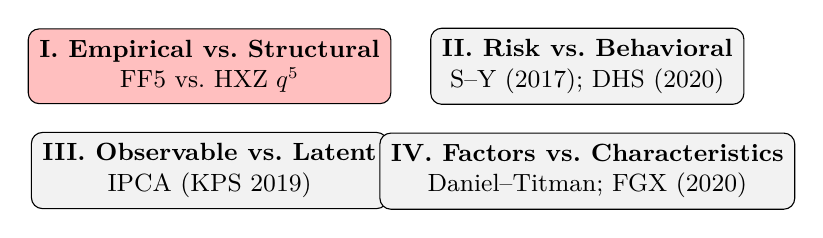
\begin{tikzpicture}[
  box/.style={draw,rounded corners,align=center,inner sep=4pt,minimum height=22pt,font=\small},
  stage/.style={box,fill=gray!10},
  here/.style={box,fill=red!25},
  node distance=10pt and 14pt]
\node[here] (b1) {\textbf{I. Empirical vs.\ Structural}\\ FF5 vs.\ HXZ $q^5$};
\node[stage,right=of b1] (b2) {\textbf{II. Risk vs.\ Behavioral}\\ S--Y (2017); DHS (2020)};
\node[stage,below=of b1] (b3) {\textbf{III. Observable vs.\ Latent}\\ IPCA (KPS 2019)};
\node[stage,below=of b2] (b4) {\textbf{IV. Factors vs.\ Characteristics}\\ Daniel--Titman; FGX (2020)};
\end{tikzpicture}
\end{center}
\begin{itemize}\small
  \item \alert{I:} \href{https://doi.org/10.1093/rof/rfy032}{\textcolor{blue}{HMXZ (2019)}} -- $q$ subsumes FF5/6 in spanning; FF reply via squared Sharpe.
  \item \alert{II:} \href{https://doi.org/10.1093/rfs/hhw107}{\textcolor{blue}{Stambaugh--Yuan (2017)}} mispricing factors; \href{https://doi.org/10.1093/rfs/hhz069}{\textcolor{blue}{Daniel--Hirshleifer--Sun (2020)}} behavioral.
  \item \alert{III:} \href{https://doi.org/10.1016/j.jfineco.2019.05.001}{\textcolor{blue}{Kelly--Pruitt--Su (2019)}} -- $\sim 5$ latent IPCA factors absorb the zoo.
  \item \alert{IV:} \href{https://doi.org/10.1111/jofi.12883}{\textcolor{blue}{Feng--Giglio--Xiu (2020)}} -- of 150+ factors, only 10--15 are genuinely useful.
\end{itemize}
\end{frame}

% =====================================================================
\subsection{China as the Cross-Section Laboratory}

\begin{frame}{China as the Cross-Section Laboratory}
China is a \alert{mechanism-testing laboratory}, not just another sample.
\begin{itemize}
  \item \textbf{Shell-value contamination:} IPO rationing inflates tiny firms, so \href{https://doi.org/10.1016/j.jfineco.2019.03.008}{\textcolor{blue}{Liu, Stambaugh, and Yuan (2019)}} drop the bottom 30\% and replace B/M with E/P. The \alert{CH3} model prices FF3, while FF3 leaves a $16.7\%$/yr alpha on the value factor (VMG).
  \item \textbf{Sentiment matters:} CH4 adds a sentiment factor (PMO), reflecting retail dominance.
  \item \textbf{Replication is brutal:} \href{https://doi.org/10.1287/mnsc.2023.4904}{\textcolor{blue}{Li, Liu, Liu, and Wei (2024)}} -- $83\%$ of 469 anomalies fail under reliable breakpoints; CH3/CH4 and the $q$-factor model perform best.
  \item \textbf{Momentum is weak, reversal dominates}; the clientele effect (\href{https://doi.org/10.1093/rof/rfac010}{\textcolor{blue}{Chui, Subrahmanyam, and Titman (2022)}}, A/B shares) ties this to who the marginal trader is.
  \item \alert{Lesson:} US-derived factors are not universal -- the cross-section must be \textbf{re-engineered} for binding short-sale limits and retail dominance.
\end{itemize}
\end{frame}

\section{The Structural Thread: ICAPM and Epstein-Zin}

\begin{frame}{Why CRRA Cannot Win: One Parameter, Two Jobs}
The structural response to the L03 puzzles starts from a single embarrassment of power utility: \alert{one parameter $\gamma$ is asked to do two unrelated jobs}.
\begin{itemize}
  \item In the CRRA SDF $m_{t+1}=\beta\,(C_{t+1}/C_t)^{-\gamma}$, the \textbf{same} $\gamma$ is both the coefficient of relative risk aversion \textit{and} the inverse of the intertemporal elasticity of substitution (IES), since $\mathrm{IES}=1/\gamma$.
  \item Taking logs, the equilibrium risk-free rate is
\end{itemize}
\begin{equation*}
  r_{f,t+1}=\underbrace{-\log\beta}_{\text{time preference}}
            +\underbrace{\gamma\,\E_t[\Delta c_{t+1}]}_{\text{intertemporal substitution }(=1/\psi\text{ should govern})}
            -\underbrace{\tfrac{\gamma^2\sigma^2_{\Delta c}}{2}}_{\text{precautionary savings}} .
\end{equation*}
\begin{block}{The straitjacket}
\textbf{Equity premium} (L03, Mehra--Prescott) needs $\gamma$ in the \alert{dozens}. But that same large $\gamma$ multiplies $\E_t[\Delta c_{t+1}]$ in $r_f$, forcing the \alert{risk-free rate far too high and too volatile} (Weil's risk-free-rate puzzle).
\end{block}
\textbf{The fix must decouple risk aversion from intertemporal substitution} -- let one parameter price gambles and a \textit{different} one govern the timing of consumption. That is exactly what \href{https://doi.org/10.2307/1913778}{\textcolor{blue}{Epstein and Zin (1989)}} deliver.
\end{frame}

\begin{frame}{The Epstein--Zin SDF, Derived (Step-by-Step)}
\small
Recursive utility separates the two jobs via a CES time aggregator over a CRRA certainty equivalent of continuation utility:
\begin{equation*}
  U_t=\Big\{(1-\delta)\,C_t^{1-1/\psi}+\delta\,\big[\E_t(U_{t+1}^{1-\gamma})\big]^{\frac{1-1/\psi}{1-\gamma}}\Big\}^{\frac{1}{1-1/\psi}},
  \qquad \theta\equiv\frac{1-\gamma}{1-1/\psi}.
\end{equation*}
Differentiate by the chain rule $C_{t+1}\!\to\! V_{t+1}\!\to\!\mu_t(V_{t+1})\!\to\! U_t$ (three derivatives: $\partial f/\partial\mu$ via $\psi$, $\partial\mu/\partial V$ via $\gamma$, $\partial V/\partial C$ via $\psi$). Collecting terms gives the \alert{primitive Epstein--Zin SDF}:
\begin{align*}
  M_{t+1}&=\delta\left(\frac{C_{t+1}}{C_t}\right)^{-1/\psi}
           \left(\frac{V_{t+1}}{\mu_t(V_{t+1})}\right)^{-(\gamma-1/\psi)} .
\end{align*}
Log-linearizing, the \textbf{SDF innovation has two pricing factors}:
\begin{align*}
  \tld{m}_{t+1}&=-\gamma\,\tld{c}_{t+1}
                 -\Big(\gamma-\tfrac{1}{\psi}\Big)\big(\tld{v}_{t+1}-\tld{c}_{t+1}\big).
\end{align*}
\begin{itemize}
  \item Factor 1: the \textbf{current consumption shock} (loading $-\gamma$).
  \item Factor 2: the \textbf{continuation-value (long-run-risk) shock} (loading $-(\gamma-1/\psi)$).
  \item \alert{When $\gamma=1/\psi$ (i.e. $\theta=1$) the second term vanishes and CRRA is recovered.} The new factor is exactly the channel CRRA cannot see.
\end{itemize}
\end{frame}

\begin{frame}{Eliminating the Unobservable: Wealth-Return Form}
The continuation value $V_{t+1}$ depends on the \textit{entire} future consumption path -- in no dataset. The \textbf{first elimination} (L09) replaces it with the wealth-portfolio return:
\begin{equation*}
  M_{t+1}=\delta^{\theta}\left(\frac{C_{t+1}}{C_t}\right)^{-\theta/\psi}\big(1+R_{W,t+1}\big)^{-(1-\theta)},
  \qquad \theta=\frac{1-\gamma}{1-1/\psi}.
\end{equation*}
\begin{block}{One family, two famous endpoints}
\begin{itemize}
  \item $\theta=1$ ($\gamma=1/\psi$): wealth term drops $\Rightarrow$ \alert{Consumption CAPM}, $M=\delta(C'/C)^{-\gamma}$.
  \item $\theta=0$ ($\gamma=1$, log utility): consumption term drops $\Rightarrow$ \alert{CAPM}, $M\propto(1+R_W)^{-1}$.
\end{itemize}
\end{block}
\begin{itemize}
  \item The SDF now uses only \textbf{consumption growth and the wealth return} -- observable in principle; CCAPM and CAPM are the \textbf{two ends of one recursive-utility family} indexed by $\theta$, not rival theories.
  \item But $R_W$ (return on \textit{all} wealth, including human capital) is itself hard to measure -- motivating a second elimination.
\end{itemize}
\end{frame}

\begin{frame}{Campbell's Consumption-Free ICAPM (Step-by-Step)}
\small
\textbf{Second elimination} (\href{https://www.jstor.org/stable/2117530}{\textcolor{blue}{Campbell (1993, 1996)}}): remove consumption via the forward-solved log-linearized budget constraint:
\begin{equation*}
  c_t-w_t=\E_t\!\left[\sum_{j=1}^{\infty}\rho^{j}\big(r_{w,t+j}-\Delta c_{t+j}\big)\right]+\frac{\rho k}{1-\rho}.
\end{equation*}
A high consumption--wealth ratio forecasts \textbf{high future returns or low consumption growth}. Substituting into $\tld m$ leaves a two-factor SDF in returns:
\begin{align*}
  \tld{m}_{t+1}&=-\gamma\,\tld{r}_{w,t+1}-(\gamma-1)\,\tld{h}_{t+1},
\end{align*}
where $\tld h_{t+1}$ is \textbf{news about future market returns}, giving the \alert{two-beta ICAPM}:
\begin{align*}
  \E_t[r_{i,t+1}]-r_{f,t+1}+\frac{\sigma_i^2}{2}
   &=\underbrace{\gamma\,\sigma_{iw}}_{\text{wealth risk, priced at }\gamma}
    +\underbrace{(\gamma-1)\,\sigma_{ih}}_{\text{intertemporal hedging, priced at }\gamma-1}.
\end{align*}
\begin{itemize}
  \item The hedging term \textbf{vanishes under log utility} ($\gamma=1$): log investors do not hedge changing opportunities.
  \item This makes \alert{``factor''} a \textbf{disciplined object}---priced factors must be innovations in state variables that \textit{forecast investment opportunities}.
\end{itemize}
\end{frame}

\begin{frame}{Taking ICAPM to Data (and to China)}
The conditional version is \href{https://doi.org/10.2307/1913811}{\textcolor{blue}{Merton's (1973)}} risk--return tradeoff -- the ``First Law of Finance'':
\begin{equation*}
  \E_t[r_{w,t+1}-r_{f,t+1}]+\frac{\sigma_m^2}{2}=\gamma\,\sigma_m^2 .
\end{equation*}
\begin{block}{Valid ICAPM state variable (\href{https://doi.org/10.1016/j.jfineco.2012.07.001}{\textcolor{blue}{Maio--Santa-Clara 2012}})}
\begin{enumerate}
  \item \textbf{forecasts} the first or second moment of aggregate returns;
  \item innovation carries a \textbf{sign-consistent} cross-sectional price of risk;
  \item implied RRA is \textbf{plausible} ($1\!-\!10$).
\end{enumerate}
\end{block}
\begin{itemize}
  \item \href{https://doi.org/10.1017/S0022109018001606}{\textcolor{blue}{Cooper and Maio (2019)}}: ICAPM is a \textbf{common background} for multifactor models -- rolling sums of factors act as state variables.
  \item Canonical state variable: \textbf{aggregate volatility} (\href{https://doi.org/10.1111/j.1540-6261.2006.00836.x}{\textcolor{blue}{Ang et al.\ 2006}}; common idiosyncratic volatility, \href{https://doi.org/10.1016/j.jfineco.2015.09.010}{\textcolor{blue}{Herskovic et al.\ 2016}}).
  \item \textbf{China} (\href{https://www.sciencedirect.com/science/article/pii/S0378426624000372}{\textcolor{blue}{Cheng, Guo and Shi 2024}}): a variance measure (MV3) plus scaled prices recovers a positive slope, $\gamma\approx4.5\!-\!8$; \alert{raw realized variance gives the wrong (negative) sign} -- omitted hedge component biases the slope.
\end{itemize}
\end{frame}

\section{The Scorecard: What Survives, What Is Contested}

\begin{frame}{Tension 1 --- Risk vs.\ Behavioral}
The deepest debate of the whole course: is the variation in $m$ a \alert{price of risk} or a \alert{belief error}? The same data fits both stories.
\begin{itemize}
  \item \textbf{Time series.} Excess volatility and predictability $=$ a rational time-varying risk premium (\href{https://onlinelibrary.wiley.com/doi/10.1111/j.1540-6261.2011.01671.x}{\textcolor{blue}{Cochrane (2011)}}) \emph{or} sentiment/bubbles (\href{http://www.jstor.org/stable/1802789}{\textcolor{blue}{Shiller (1981)}}). The Campbell--Shiller decomposition is an identity: it stays agnostic.
  \item \textbf{Value.} Distress-risk compensation (\href{https://doi.org/10.1111/j.1540-6261.1996.tb05202.x}{\textcolor{blue}{Fama--French (1996)}}) \emph{or} overreaction to past growth (\href{https://doi.org/10.1111/j.1540-6261.1994.tb04772.x}{\textcolor{blue}{Lakonishok, Shleifer, Vishny (1994)}}).
  \item \textbf{Momentum / IVOL.} $q$-theory and growth-rate risk \emph{or} under/overreaction and lottery demand --- both readings survive (\href{https://doi.org/10.1111/j.1540-6261.2006.00836.x}{\textcolor{blue}{Ang et al.\ (2006)}}).
  \item \textbf{Why it cannot be settled on the cross-section.} \href{https://doi.org/10.1111/jofi.12612}{\textcolor{blue}{Kozak, Nagel, Santosh (2018)}}: absent near-arbitrage, \emph{any} admissible SDF --- rational \emph{or} behavioral --- is spanned by a few dominant PCs. A tidy factor model is observationally near-identical under both camps.
\end{itemize}
\begin{block}{Verdict}
\textbf{Unresolved by the cross-section alone.} Adjudication needs out-of-sample discipline and direct \emph{beliefs data} (surveys, analyst forecasts) --- a Frontier IV question.
\end{block}
\end{frame}

\begin{frame}{Tension 2 --- Structural Theory vs.\ Reduced-Form Factors}
\small
Where should the factors in $m$ \emph{come from} --- an ex-post empirical patch, or an ex-ante primitive model?
\begin{itemize}
  \item \textbf{The split (Lec.\ 05--07).} FF camp: add mimicking portfolios, justified ex post (\href{https://doi.org/10.1016/j.jfineco.2014.10.010}{\textcolor{blue}{Fama--French (2015)}}); Zhang camp: derive factors from the firm's investment FOC (\href{https://doi.org/10.1093/rfs/hhu068}{\textcolor{blue}{Hou, Xue, Zhang (2015)}}).
  \item \textbf{The structural pole.} ICAPM / Epstein--Zin \emph{microfound} $m$: priced factors are innovations in state variables forecasting investment opportunities (\href{https://doi.org/10.2307/1913811}{\textcolor{blue}{Merton (1973)}}); the zoo just reverse-engineers the same $m$. \href{https://doi.org/10.1017/S0022109018001606}{\textcolor{blue}{Cooper--Maio (2019)}}: ICAPM licenses multifactor models via rolling factor sums as state variables.
  \item \textbf{The catch.} Even ``structural'' models smuggle in reduced-form choices: the $q^5$ growth factor $R_{\mathrm{Eg}}$ is \emph{constructed}, depending on the predictor list and weakening if operating cash flows are dropped (\href{https://doi.org/10.1093/rof/rfaa004}{\textcolor{blue}{Hou, Mo, Xue, Zhang (2021)}}).
\end{itemize}
\begin{block}{Verdict}
A \textbf{hybrid consensus}: discipline reduced-form factors with theory (valid ICAPM state variables, the investment FOC), but concede no model is purely structural.
\end{block}
\end{frame}

\begin{frame}{Tension 3 --- US vs.\ China, and the Replication Crisis}
Does the cross-section travel? Two stress tests of external validity.
\begin{columns}[T]
\begin{column}{0.5\textwidth}
\textbf{The credibility revolution}
\begin{itemize}\small
  \item \href{https://doi.org/10.1093/rfs/hhy131}{\textcolor{blue}{Hou, Xue, Zhang (2020)}}: $\sim$65\% of 452 anomalies fail under value-weighting and microcap exclusion.
  \item \href{https://doi.org/10.1093/rfs/hhv059}{\textcolor{blue}{Harvey, Liu, Zhu (2016)}}: with 300+ tests, the bar is $t>3.0$.
  \item \href{https://doi.org/10.1111/jofi.12365}{\textcolor{blue}{McLean--Pontiff (2016)}}: $\sim$26\% post-publication decay.
\end{itemize}
\end{column}
\begin{column}{0.5\textwidth}
\textbf{China as out-of-sample test}
\begin{itemize}\small
  \item Most US factors fail (\href{https://doi.org/10.1016/j.jfineco.2019.03.008}{\textcolor{blue}{Liu, Stambaugh, Yuan (2019)}}; \href{https://doi.org/10.1287/mnsc.2023.4904}{\textcolor{blue}{Li et al.\ (2024)}}: $83\%$ fail).
  \item Shell-value premium, reversal $>$ momentum, retail dominance force a redesigned recipe.
\end{itemize}
\end{column}
\end{columns}
\vspace{4pt}
\begin{block}{The reconciling result}
\href{https://doi.org/10.1111/jofi.13249}{\textcolor{blue}{Jensen, Kelly, Pedersen (2023)}}: across 93 countries, factor \emph{families} replicate robustly even where \emph{individual} factors do not --- a stable global core under the noise.
\end{block}
\centerline{\textbf{Verdict: a small core survives; market structure (who trades, what they can short) matters.}}
\end{frame}

\begin{frame}{Synthesis Scorecard: The Robust Core}
What the profession provisionally agrees on, viewed through $1 = \E_t[m\,R]$.
\vspace{2pt}
\begin{center}\footnotesize
\begin{tabular}{@{}p{0.30\textwidth}p{0.30\textwidth}p{0.30\textwidth}@{}}
\toprule
\textbf{Robust core factors} & \textbf{Robust facts} & \textbf{Open (define Frontiers)} \\
\midrule
Market, size, value, profitability, investment & Discount rates vary (predictability real but \emph{modest} OOS) & \alert{Source of $m$}: risk vs.\ belief \\
Momentum \textit{(with crash caveats)} & Cross-section is \emph{low-dimensional} & How \emph{many} factors? \\
$+$ a few latent factors (PCA/IPCA) & Equity premium puzzle still binds CRRA & Term structure of equity \\
 & $m$ is \emph{dense} in characteristic space & Structural microfoundation of $m$ \\
\bottomrule
\end{tabular}
\end{center}
\vspace{3pt}
\begin{block}{Bridge to the Frontiers}
\alert{The open items \emph{are} the five frontiers}: disciplined SDF estimation, machine learning, intermediary/demand-based pricing, behavioral beliefs, and consumption-macro engines taking Epstein--Zin to data.
\end{block}
\end{frame}

\section{Frontier I - Estimating the SDF and Disciplining the Factor Zoo}

\begin{frame}{Reframing: From ``Which Factors?'' to ``Estimate $m$''}
\begin{block}{The pivot}
Stop asking \alert{``which named factors enter the model?''}\\
Start asking \alert{``how do we \textbf{estimate the SDF $m$ itself}, with enough discipline not to overfit?''}
\end{block}
\textbf{Why this is the same question} (recall Lecture 03): the SDF representation is mathematically \textit{equivalent} to an expected-return--beta model,
\begin{equation*}
1 = \E_t[\,m_{t+1}\, R_{t+1}\,]
\quad\Longleftrightarrow\quad
\E[R^e_i] = \beta_i'\lambda .
\end{equation*}
\begin{itemize}
\item So \alert{``estimate $m$''} and \alert{``select factors''} are \textbf{literally the same problem}.
\end{itemize}
\textbf{The disease} (Lecture 07 recap):
\begin{itemize}
\item \href{https://doi.org/10.1093/rfs/hhv059}{\textcolor{blue}{Harvey, Liu, and Zhu (2016)}}: $316{+}$ published ``factors.''
\item Run $300$ independent tests and some clear $t=1.96$ \textbf{by pure luck}.
\item Any fixed $5$- or $6$-factor model is just \textbf{one sparse guess} at a high-dimensional object $m$.
\end{itemize}
\end{frame}

\begin{frame}{Three Disciplines: Multiple Testing, Spanning, Shrinkage}
\small
\begin{block}{Discipline 1 --- Multiple testing}
A single $t$-stat is meaningless after hundreds of tests.
\begin{itemize}
\item \href{https://doi.org/10.1093/rfs/hhv059}{\textcolor{blue}{Harvey, Liu, and Zhu (2016)}}: false-discovery logic $\Rightarrow$ raise the bar to $t > 3.0$.
\item \href{https://doi.org/10.1111/jofi.12530}{\textcolor{blue}{Harvey (2017)}}: the zoo is a \textit{p-hacking / publication-incentive} crisis --- bad scientific method, not bad economics.
\end{itemize}
\end{block}
\begin{block}{Discipline 2 --- Spanning \& max-Sharpe}
The SDF \textit{is} the max-Sharpe portfolio $\Rightarrow$ the best model maximizes factors' squared Sharpe ratio.
\begin{itemize}
\item \href{https://doi.org/10.1093/rfs/hhw101}{\textcolor{blue}{Barillas and Shanken (2017)}}: \textbf{test assets are irrelevant} --- only factors' max $SR^2$ matters.
\item \href{https://doi.org/10.1111/jofi.12607}{\textcolor{blue}{Barillas and Shanken (2018)}}: rank by \textbf{Bayesian posterior}, with a built-in complexity penalty.
\end{itemize}
\end{block}
\begin{block}{Discipline 3 --- Shrinkage (the key move)}
\href{https://doi.org/10.1016/j.jfineco.2019.06.008}{\textcolor{blue}{Kozak, Nagel, and Santosh (2020)}}: the SDF is \alert{dense} in characteristic space --- not variable selection but economically-motivated shrinkage.
\end{block}
\end{frame}

\begin{frame}{Discipline 3, Unpacked: Why Shrink Toward High-Variance PCs}
\textbf{Setup.} Build $m$ from $N$ characteristic-managed portfolio returns $R$, projected onto principal components $P_1,\dots,P_N$ (ordered by eigenvalue / variance):
\begin{equation*}
m_{t+1} = 1 - b'\big(R_{t+1} - \E[R_{t+1}]\big), \qquad R = \textstyle\sum_k P_k .
\end{equation*}
\textbf{No-near-arbitrage bound.} A finite maximum Sharpe ratio caps how hard $m$ can load on \alert{low-variance} PCs:
\begin{align*}
SR^2_{\max} &= \sum_{k=1}^{N} \frac{(\text{PC-}k \text{ mean})^2}{\lambda_k} \;<\; \infty
\quad\Longrightarrow\quad
\text{small } \lambda_k \Rightarrow \text{tiny priced mean.}
\end{align*}
\begin{itemize}
\item A large $b$ on a tiny-variance PC implies a near-arbitrage --- economically implausible --- so \textbf{shrink SDF coefficients toward zero on low-eigenvalue PCs}.
\end{itemize}
\begin{block}{The estimator}
A \textbf{Bayesian prior} down-weighting low-variance PCs $\;\Rightarrow\;$ ridge/lasso (elastic-net) shrinkage toward \alert{high-eigenvalue} PCs. Pure sparsity (a few named factors) \textbf{fails out-of-sample}; the dense, shrunk SDF \textbf{wins}.
\end{block}
\end{frame}

\begin{frame}{The Yardstick: Hansen--Jagannathan Distance}
\begin{block}{The grading tool: Hansen--Jagannathan distance}
\href{https://doi.org/10.1111/j.1540-6261.1997.tb04813.x}{\textcolor{blue}{Hansen and Jagannathan (1997)}} --- least-squares distance from a candidate $m$ to the true pricing kernels:
\begin{equation*}
\delta_{HJ} = \min_{m^{\ast}}\; \big\|\, m - m^{\ast} \,\big\|, \qquad m^{\ast}\in\{\text{true kernels}\}.
\end{equation*}
\begin{itemize}
\item Comparable across models; unlike a GMM $J$-stat, \textbf{does not reward noisy SDFs}.
\item HJ bound (Lec.\ 03): $\;\dfrac{\sigma(m)}{\E(m)} \ge \dfrac{|\E[R^e]|}{\sigma(R^e)} = |SR(R^e)|$.
\end{itemize}
\end{block}
\end{frame}

\begin{frame}{The Emerging Consensus}
\textbf{Where the field has landed:}
\begin{itemize}
\item A \textbf{few latent factors} on a \textbf{wide} characteristic set \textbf{plus shrinkage} beats any fixed named model OOS --- PCA, \href{https://doi.org/10.1016/j.jfineco.2019.05.001}{\textcolor{blue}{Kelly, Pruitt, and Su (2019)}} IPCA, Lettau--Pelger PCA-RP.
\item \href{https://doi.org/10.1111/jofi.12612}{\textcolor{blue}{Kozak, Nagel, and Santosh (2018)}}: a low-dim factor structure fits \textbf{both} risk \textbf{and} behavioral stories --- ``characteristics price the cross-section'' and ``a low-dim covariance spans $m$'' are \textit{not} contradictory.
\end{itemize}
\begin{block}{China angle}
Short samples $+$ data-mining risk $+$ a different anomaly set $\Rightarrow$ shrinkage / latent-factor SDFs are the right default; transplanting US named factors (FF5, $q$-factor) is statistically unjustified.
\end{block}
\end{frame}

\section{Frontier II - Machine Learning and Big Data}

\begin{frame}{ML as Flexible Estimation of \texorpdfstring{$\E_t[R]$}{Et[R]} and \texorpdfstring{$m$}{m}}
The master equation is \emph{unchanged}; machine learning is the constructive response to the Lecture 07 factor-zoo crisis.
\begin{equation*}
1 = \E_t\!\left[\, m_{t+1}\, R_{t+1}\,\right]
\end{equation*}
ML attacks the two objects the linear factor program left \alert{ill-posed}:
\begin{itemize}
  \item \textbf{The conditional mean} $\E_t[R_{t+1}] = f(z_{i,t})$, where $z_{i,t}$ stacks \emph{hundreds} of firm characteristics and macro state variables --- with \alert{unknown nonlinearities and interactions}:
  \begin{equation*}
    \E_t[R_{i,t+1}] = f\big(\underbrace{x_{i,t}}_{\text{100s of chars}},\ \underbrace{s_t}_{\text{macro state}}\big), \qquad f \text{ unknown}.
  \end{equation*}
  \item \textbf{The latent SDF} $m_{t+1}$ itself, estimated flexibly from a wide cross-section of characteristic-managed returns under a no-arbitrage discipline.
\end{itemize}
\begin{block}{The unifying methodological move}
Economic structure --- no-arbitrage, a \emph{low-dimensional} SDF, a Sharpe-ratio prior --- enters as \alert{regularization}, \textit{not} as a maintained functional form. Estimating $m$ and ``finding the right factors'' are the same problem (Lecture 03: $1=\E(mR)$ is equivalent to a beta-pricing model).
\end{block}
\end{frame}

\begin{frame}{The Empirical Verdict and the Two Branches}
\textbf{The horse race --- \href{https://doi.org/10.1093/rfs/hhaa009}{\textcolor{blue}{Gu, Kelly, and Xiu (2020)}}:}
\begin{itemize}
  \item OLS vs.\ elastic net, PCR/PLS, random forests, boosted trees, neural nets on the US monthly cross-section.
  \item Nets and trees roughly \alert{double} out-of-sample $R^2$ and lift long-short Sharpe ratios sharply.
  \item Gains come from \textbf{nonlinearities and interactions} among a \emph{few dominant} signals (momentum, liquidity, volatility) --- not new characteristics.
\end{itemize}
\textbf{The latent-factor branches} (let data map characteristics into the SDF):
\begin{itemize}
  \item \href{https://doi.org/10.1016/j.jfineco.2019.05.001}{\textcolor{blue}{Kelly, Pruitt, and Su (2019)}} --- \alert{IPCA}: ``characteristics \emph{are} covariances,'' betas \emph{linear} in $z_{i,t}$:
  \begin{equation*}
    R_{i,t+1} = \beta_{i,t}'\, f_{t+1} + \varepsilon_{i,t+1}, \qquad \beta_{i,t} = z_{i,t}'\,\Gamma .
  \end{equation*}
  \item \href{https://doi.org/10.1016/j.jeconom.2020.07.009}{\textcolor{blue}{Gu, Kelly, and Xiu (2021)}} --- \alert{conditional autoencoder}: \emph{nonlinear} factors and loadings via a no-arbitrage neural net.
  \item \href{https://doi.org/10.1093/rfs/hhz123}{\textcolor{blue}{Freyberger, Neuhierl, and Weber (2020)}} --- nonparametric joint \emph{selection} (adaptive group LASSO + splines): many characteristics are redundant once nonlinearity is allowed.
\end{itemize}
\end{frame}

\begin{frame}{Estimating \texorpdfstring{$m$}{m} Directly, and the Cost of Black Boxes}
\small
\textbf{The SDF as the estimand --- \href{https://doi.org/10.1287/mnsc.2023.4695}{\textcolor{blue}{Chen, Pelger, and Zhu (2024)}}:} estimate $m$ \emph{directly} with a deep net under no-arbitrage, so $m$ is the object, not a residual:
\begin{equation*}
  \E\!\left[\, m_{t+1}\, R^e_{i,t+1}\, g(z_{i,t})\,\right] = 0 \quad \forall\, g .
\end{equation*}
A \alert{GAN}/adversarial step finds the \emph{hardest} conditioning $g(\cdot)$; an LSTM summarizes macro states $s_t$.

\textbf{The economic prior \emph{is} shrinkage --- \href{https://doi.org/10.1016/j.jfineco.2019.06.008}{\textcolor{blue}{Kozak, Nagel, and Santosh (2020)}}:} ``implausibly large Sharpe ratios'' becomes an elastic-net penalty; the no-arbitrage $m$ is \alert{sparse in PC space}, explaining the zoo's low effective dimension.
\begin{block}{The central tension --- predictive power vs.\ interpretability}
Black-box gains are real but fragile: report \alert{OOS $R^2$ and net-of-cost Sharpe}, never in-sample fit. Guard against data snooping (\href{https://doi.org/10.1093/rfs/hhv059}{\textcolor{blue}{Harvey, Liu, and Zhu (2016)}}), transaction costs, and post-publication decay. \alert{Alt data \& LLMs} (text, satellite, card) widen $X$ but invite look-ahead contamination; \textbf{China} --- short samples, retail/sentiment share, breaks --- makes OOS fragility acute, so stress-test before reading ML gains as risk premia.
\end{block}
\end{frame}

\section{Frontier III - Intermediary Asset Pricing, Frictions, and Demand Systems}

\begin{frame}{Who Is the Marginal Investor? Re-Specifying $m$}
\textbf{The problem.} The consumption-CAPM of Lecture 03 prices the cross-section \emph{only} if households are marginal --- but aggregate consumption is far too smooth and too weakly correlated with returns to rationalize observed premia (the equity-premium puzzle).
\begin{itemize}
  \item \textbf{Markets are intermediated.} Assets are priced at the margin by \alert{leveraged, constrained intermediaries}: broker-dealers, hedge funds, primary dealers.
  \item \textbf{Same equation, new kernel.} Keep the master Euler equation but re-specify \emph{whose} marginal value of wealth $m$ is:
  \begin{equation*}
    1 = \E_t\!\left[\, m_{t+1}\, R_{t+1}\,\right],
    \qquad
    m_{t+1} = \underbrace{\frac{\text{intermediary's marginal value of wealth}}{\text{(constrained)}}}_{\text{not household marginal utility of } C}
  \end{equation*}
\end{itemize}
\end{frame}

\begin{frame}{Who Is the Marginal Investor? The Pricing Mechanism}
\textbf{Recap.} Same Euler equation $1 = \E_t[\, m_{t+1}\, R_{t+1}\,]$, but $m$ is now the \alert{constrained intermediary's} marginal value of wealth --- not household marginal utility of consumption.
\begin{itemize}
  \item \textbf{The story.} When intermediary capital is \alert{scarce}, the constraint binds, $m$ spikes, and premia rise --- $m$ becomes a function of an \textit{observable} state (intermediary leverage or equity capital ratio).
\end{itemize}
\begin{block}{The conceptual move}
This turns \textbf{limits to arbitrage} (mispricing persists because arbitrageurs are capital-constrained) from a friction that \emph{breaks} pricing into the pricing \alert{mechanism itself}.
\end{block}
\end{frame}

\begin{frame}{From Theory to a Measurable Intermediary Factor}
\begin{block}{Structural foundation}
\href{https://doi.org/10.1257/aer.103.2.732}{\textcolor{blue}{He and Krishnamurthy (2013)}}: specialists face an \textbf{equity capital constraint}. When capital is scarce it binds and risk premia rise \alert{nonlinearly} --- a structural theory of crisis-time discount rates.
\end{block}
\textbf{Making $m$ observable.} The model says the intermediary's marginal value of wealth drives risk premia. To take this to data, proxy that latent quantity by a \emph{measurable} state variable describing intermediary health.
\begin{itemize}
  \item When intermediary capital is abundant, the constraint slacks and the marginal value of wealth is low.
  \item When capital is scarce (deleveraging, equity erosion), it binds and the marginal value of wealth spikes $\Rightarrow$ high risk prices.
\end{itemize}
\end{frame}

\begin{frame}{A Measurable Intermediary Factor: Evidence}
\textbf{Two empirical proxies for $m$:}
\begin{itemize}
  \item \href{https://doi.org/10.1111/jofi.12189}{\textcolor{blue}{Adrian, Etula, and Muir (2014)}}: shocks to broker-dealer \textbf{leverage}. A \emph{single} factor prices size, value, momentum, and bonds ($R^2 \approx 77\%$, pricing error $\approx 1\%$), rivaling multifactor benchmarks. Deleveraging $=$ high marginal value of wealth.
  \item \href{https://doi.org/10.1016/j.jfineco.2017.08.002}{\textcolor{blue}{He, Kelly, and Manela (2017)}}: shocks to the primary-dealer equity \textbf{capital ratio} carry a \alert{positive} price of risk across equities, bonds, options, CDS, commodities, and FX --- broadest cross-asset evidence for a common marginal investor.
\end{itemize}
\begin{tcolorbox}[colback=postit,colframe=red!60!black,title=Live measurement debate]
Dealer \textbf{leverage} (procyclical, AEM) and the equity \textbf{capital ratio} (HKM) can move in \alert{opposite} directions --- ``measuring intermediary health'' is itself contested.
\end{tcolorbox}
\end{frame}

\begin{frame}{Frictions and Demand-System Pricing}
\textbf{Funding frictions as the price of risk.}
\begin{itemize}
  \item \href{https://doi.org/10.1093/rfs/hhn098}{\textcolor{blue}{Brunnermeier and Pedersen (2009)}}: \textbf{funding} and \textbf{market liquidity} reinforce each other $\rightarrow$ \alert{liquidity spirals}, flight to quality. Arbitrageur capital \textbf{is} the SDF.
\end{itemize}
\textbf{Demand systems: drop the single Euler equation.}
\begin{itemize}
  \item \href{https://doi.org/10.1086/701683}{\textcolor{blue}{Koijen and Yogo (2019)}}: price $=$ \alert{fixed point} of investors' characteristic-based demand, estimated from 13F holdings via IV. Asks \emph{who} holds an asset and \emph{why}.
  \item \href{https://doi.org/10.3386/w28967}{\textcolor{blue}{Gabaix and Koijen (2021)}}, inelastic markets: \$1 of flow moves market cap by $\approx$\$5. \textbf{Flows move prices}; fluctuations originate in intermediated demand, not cash-flow news.
\end{itemize}
\begin{block}{Frontier tension + China}
\textbf{One marginal investor?} \href{https://doi.org/10.1111/jofi.13469}{\textcolor{blue}{Siriwardane, Sunderam, and Wallen (2025)}}: arbitrage is \alert{segmented} across trades (CIP, equity-spot-futures, TIPS-Treasury), against a common intermediary SDF. \textbf{China:} bank-dominated intermediation, the leverage-driven 2015 boom-bust, and concentrated holdings make these lenses apt.
\end{block}
\end{frame}

\section{Frontier IV - Behavioral, Subjective Expectations, and New Asset Classes}

\begin{frame}{Whose Expectation Is $\E_t$? Beliefs Inside the SDF}
\begin{block}{The hidden choice in the master equation}
\begin{equation*}
1 = \E_t\!\left[ m_{t+1}\, R_{t+1} \right]
\end{equation*}
This course estimated $m$ while \alert{taking $\E_t$ for granted}. The frontier asks: \textbf{whose} expectation -- the econometrician's \textit{rational} operator, or investors' \textit{subjective} one?
\end{block}
\begin{itemize}
  \item Replace $\E_t$ with \textbf{measured} subjective expectations (surveys, analyst forecasts): they diverge \textit{systematically} from the rational benchmark.
  \item \href{https://doi.org/10.1093/rfs/hht082}{\textcolor{blue}{Greenwood and Shleifer (2014)}}: across six surveys, expected returns are high precisely when \textit{objective} returns are \alert{low}. Investors \textbf{extrapolate}: high prices reflect \alert{optimism}, not low required returns.
  \item So part of the ``risk premium'' in $m$ is a \alert{belief wedge}: \quad $\underbrace{\E_t^{\text{rational}}[R]}_{\text{required return}} \;\neq\; \underbrace{\widehat{\E}_t^{\text{survey}}[R]}_{\text{investors expect}}$
  \item The missing \textit{micro-foundation} for the \textbf{excess volatility} puzzle (L01): \alert{beliefs} move more than fundamentals.
\end{itemize}
\end{frame}

\begin{frame}{Diagnostic Expectations: A Portable Engine for Belief Errors}
\begin{block}{Representativeness made dynamic}
\href{https://doi.org/10.1111/jofi.12586}{\textcolor{blue}{Bordalo, Gennaioli, and Shleifer (2018)}} -- \textbf{diagnostic expectations}: representativeness made dynamic. Agents over-weight states whose likelihood news just rose $\Rightarrow$ \alert{over-reaction}, then \alert{predictable reversal}.
\end{block}
\begin{itemize}
  \item \textbf{Cross-section test} -- \href{https://doi.org/10.1111/jofi.12833}{\textcolor{blue}{Bordalo, Gennaioli, La Porta, and Shleifer (2019)}}: optimistic long-term growth forecasts predict \alert{under}-performance. \textit{Belief errors}, not risk, drive much cross-sectional predictability.
  \item Tempting to settle the L04 anomaly debate by matching expectation errors to returns -- but a deeper result blocks a clean verdict.
\end{itemize}
\end{frame}

\begin{frame}{Why the Cross-Section Alone Cannot Settle the Verdict}
\begin{block}{Near-arbitrage pins the SDF to a few PCs}
\href{https://doi.org/10.1111/jofi.12612}{\textcolor{blue}{Kozak, Nagel, and Santosh (2018)}}: absence of near-arbitrage forces \textit{any} admissible SDF onto a few dominant PCs:
\begin{equation*}
m_{t+1} = 1 - \sum_{j=1}^{K} b_j\, F_{j,t+1}, \qquad F_j = \text{high-variance PCs of returns.}
\end{equation*}
A low-dimensional factor SDF fits \textbf{both} a \alert{risk} and a \alert{sentiment} story -- observationally \textbf{near-identical}. The debate is \alert{not} settled by the cross-section alone.
\end{block}
\end{frame}

\begin{frame}{New Asset Classes Discipline the Kernel}
\small
Beyond U.S.\ equities, fresh \textbf{test assets} pin down what $m$ can be -- progress now comes from \alert{new data}, not another factor.
\begin{block}{Climate, intangibles, crypto}
\begin{itemize}
  \item \textbf{Climate:} \href{https://doi.org/10.1016/j.jfineco.2021.05.008}{\textcolor{blue}{Bolton and Kacperczyk (2021)}} -- a \alert{carbon premium}: high-emission firms earn higher returns. Climate is a priced transition state; news-hedging gives a new $\beta$.
  \item \textbf{Intangibles:} \href{https://www.nber.org/papers/w28056}{\textcolor{blue}{Eisfeldt, Kim, and Papanikolaou (2022)}} -- capitalizing intangibles into book equity \alert{partly revives} value. ``Death of value'' is mostly \textbf{mismeasurement}.
  \item \textbf{Crypto:} a novel class with its own factors (size, momentum, network), 24/7 -- a live test of whether \textit{known} factors price \textit{novel} assets.
\end{itemize}
\end{block}
\begin{block}{China as a natural experiment}
\href{https://doi.org/10.1016/j.jfineco.2019.03.008}{\textcolor{blue}{Liu, Stambaugh, and Yuan (2019)}}: high retail share, short-sale limits, and shell-firm contamination make China a lab for \textbf{separating} risk vs.\ preference vs.\ slow correction -- drop the smallest 30\%, use E/P, and the local factors re-engineer the U.S.\ recipe.
\end{block}
\end{frame}

\section{Frontier V - Consumption-Based Macro Engines (The Theory Frontier)}

\begin{frame}{Three Stories About $m$, One Equation}
\justifying
The whole course is $1=\E_t[m_{t+1}R_{t+1}]$. The plain CRRA consumption SDF tells the simplest story --- and it fails:
\begin{equation*}
m_{t+1}=\beta\left(\frac{C_{t+1}}{C_t}\right)^{-\gamma},\qquad
\E_t[r^e_{i,t+1}]+\tfrac{\sigma_i^2}{2}=\gamma\,\sigma_{ic}.
\end{equation*}
Matching a $\sim 6\%$ premium needs $\gamma>30$, which then forces a counterfactually high, volatile $r_f$ (\href{https://www.sciencedirect.com/science/article/pii/0304393285900613}{\textcolor{blue}{Mehra--Prescott (1985)}} / \href{https://doi.org/10.1016/0304-3932(89)90028-7}{\textcolor{blue}{Weil (1989)}}).
\begin{block}{The theory frontier: three structural rescues, $\gamma\approx 2$--$10$}
Three macro engines fix the \emph{story about $m$} without an absurd $\gamma$.
\end{block}
\begin{itemize}\small
\item \textbf{(1) Long-run risk} (\href{https://doi.org/10.1111/j.1540-6261.2004.00670.x}{\textcolor{blue}{Bansal--Yaron (2004)}}): a small, highly \emph{persistent} component $x_t$ in expected growth, plus time-varying volatility $\sigma_t^2$, priced by Epstein--Zin.
\item This is exactly the L08--09 engine instantiated: the SDF prices \alert{news about future growth}, the $-(\gamma-\tfrac{1}{\psi})\,\tld{g}_{t+1}$ term.
\item \textbf{(2) Habit} and \textbf{(3) rare disasters} --- next slide.
\end{itemize}
\end{frame}

\begin{frame}{Long-Run Risk: How Persistence Amplifies $m$}
\justifying
Recall the L09 Campbell-form Epstein--Zin SDF innovation and its risk-premium decomposition:
\begin{align*}
\tld{m}_{t+1} &= -\gamma\,\tld{c}_{t+1}-\Big(\gamma-\tfrac{1}{\psi}\Big)\,\tld{g}_{t+1},\\
\E_t[r^e_{i,t+1}]+\tfrac{\sigma_i^2}{2}
 &= \gamma\,\sigma_{ic}+\Big(\gamma-\tfrac{1}{\psi}\Big)\,\sigma_{ig}.
\end{align*}
The state evolves with a near-unit-root growth component:
\begin{equation*}
\Delta c_{t+1}=\mu+x_t+\sigma_t\,\eta_{t+1},\qquad
x_{t+1}=\rho_x\,x_t+\varphi\,\sigma_t\,e_{t+1},\quad \rho_x\approx 0.98 .
\end{equation*}
The price-consumption coefficient on $x_t$ blows up with persistence:
\begin{equation*}
A_1=\frac{1-\tfrac{1}{\psi}}{1-\kappa_1\,\rho_x}
\;\xrightarrow{\ \rho_x\to 1\ }\ \text{large.}
\end{equation*}
\begin{itemize}\small
\item With $\psi>1$ and $\gamma>1/\psi$, a tiny but persistent shock to $x_t$ moves \alert{wealth} a lot --- a large $\sigma_{ig}$ and hence a large premium at $\gamma\approx 10$.
\item Adding $\sigma_t^2$ as a second state delivers \alert{time-varying} premia, predictability, and excess volatility.
\end{itemize}
\end{frame}

\begin{frame}{Habit and Rare Disasters}
\justifying
The other two engines keep \emph{power utility} but change a different ingredient.
\begin{block}{(2) External habit --- \href{https://doi.org/10.1086/250059}{\textcolor{blue}{Campbell--Cochrane (1999)}}}
Utility over the gap $C_t-X_t$, with $X_t$ a slow-moving \emph{external} habit. Define the surplus consumption ratio $S_t=(C_t-X_t)/C_t$. Local curvature --- effective risk aversion --- is
\begin{equation*}
\eta_t \equiv -\frac{C_t\,u''}{u'}=\frac{\gamma}{S_t},
\end{equation*}
which is \alert{high and countercyclical}: $S_t$ falls in recessions, so $\eta_t$ spikes exactly when consumption is low. No EIS gymnastics needed.
\end{block}
\begin{block}{(3) Rare disasters --- \href{https://doi.org/10.1016/0304-3932(88)90172-9}{\textcolor{blue}{Rietz (1988)}}; \href{https://doi.org/10.1162/qjec.121.3.823}{\textcolor{blue}{Barro (2006)}}; \href{https://doi.org/10.1111/jofi.12018}{\textcolor{blue}{Wachter (2013)}}}
Normal times look benign, but consumption carries a small probability $p$ of a large crash. The premium is \alert{crash insurance}; \href{https://doi.org/10.1111/jofi.12018}{\textcolor{blue}{Wachter (2013)}} makes $p_t$ time-varying, adding volatility and predictability.
\end{block}
\centerline{\small\textbf{Common scorecard:} high premium, low/stable $r_f$, P/D predictability, excess volatility --- all at $\gamma\approx 2$--$10$.}
\end{frame}

\begin{frame}{Same Fact, Three Engines}
\justifying
All three explain \alert{countercyclical risk premia} --- but locate the time-variation in a different state.
\begin{center}
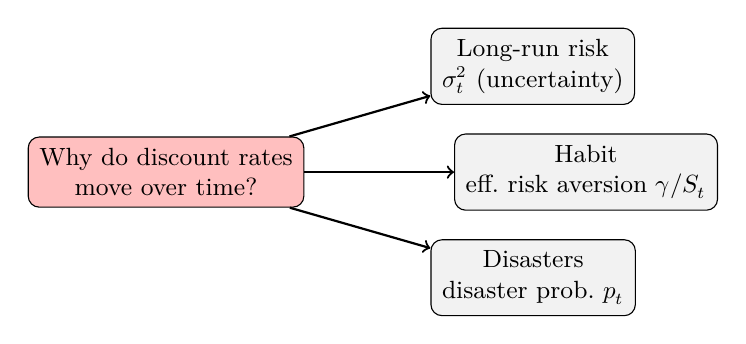
\begin{tikzpicture}[
  box/.style={draw,rounded corners,align=center,inner sep=4pt,minimum height=22pt,font=\small},
  stage/.style={box,fill=gray!10},
  here/.style={box,fill=red!25}]
\node[here] (q) {Why do discount rates\\ move over time?};
\node[stage,above right=0.4cm and 1.6cm of q] (lrr) {Long-run risk\\ $\sigma_t^2$ (uncertainty)};
\node[stage,right=1.9cm of q] (hab) {Habit\\ eff.\ risk aversion $\gamma/S_t$};
\node[stage,below right=0.4cm and 1.6cm of q] (dis) {Disasters\\ disaster prob.\ $p_t$};
\draw[thick,->] (q) -- (lrr);
\draw[thick,->] (q) -- (hab);
\draw[thick,->] (q) -- (dis);
\end{tikzpicture}
\end{center}
\begin{itemize}\small
\item \textbf{Time series} (L02): three structural microfoundations for the reduced-form predictability of L01--02.
\item \textbf{Cross section} (L05--07): long-run risk maps cash-flow \alert{duration} to a long-run-risk beta --- a structural value-premium story; habit and disasters are weaker cross-sectionally.
\item These are the \alert{structural} pole of the structural-vs-reduced-form tension: they \emph{microfound} the $m$ that the factor zoo only reverse-engineers.
\end{itemize}
\end{frame}

\begin{frame}{Where They Diverge: Discriminating Tests}
\justifying
Same scorecard, but the engines make \emph{different} predictions where it counts.
\begin{enumerate}\small
\item \textbf{Equity term structure / dividend strips.} Standard long-run risk and habit imply an \alert{upward}-sloping term structure of equity; the data (\href{https://doi.org/10.1257/aer.102.4.1596}{\textcolor{blue}{van Binsbergen--Brandt--Koijen (2012)}}) suggest short-horizon claims earn high returns --- a \alert{downward} short end. A live challenge.
\item \textbf{Options \& the variance risk premium.} Disasters naturally generate fat left tails and expensive put protection; long-run risk works through vol-of-vol. The VRP discriminates.
\item \textbf{Cross-section.} Only long-run risk ties cash-flow \alert{duration} to a structural beta, linking back to the value premium of L05--07.
\end{enumerate}
\begin{block}{Empirical pushback --- \href{https://doi.org/10.1561/104.00000004}{\textcolor{blue}{Beeler--Campbell (2012)}}}
The near-unit-root $x_t$ is essentially \alert{unidentifiable} in short consumption samples (looks like $\rho_x=1$); the model over-predicts cash-flow predictability; and it needs $\psi>1$ while many micro estimates find $\psi<1$ --- the macro-vs-micro EIS puzzle. Rebuttal: \href{https://doi.org/10.1561/104.00000005}{\textcolor{blue}{Bansal--Kiku--Yaron (2012)}}.
\end{block}
\centerline{\small \textit{Open question:} can $x_t$, $p_t$, and a random walk ever be told apart in the data we actually have?}
\end{frame}

\section{Closing: Open Questions and How to Do the Research}

\begin{frame}{The Grand Open Questions}
We have re-derived $1=\E_t[m_{t+1}R_{t+1}]$ nine times and toured five frontiers. Here is what is \alert{still unsettled} -- and where you come in.
\begin{enumerate}
  \item \textbf{Risk vs.\ belief.} Once $m$ is a \emph{statistical} object (a few dominant PCs), a low-dimensional kernel fits \alert{both} rational and behavioral stories (\href{https://doi.org/10.1111/jofi.12612}{\textcolor{blue}{Kozak--Nagel--Santosh (2018)}}). What evidence \emph{beyond pricing fit} can adjudicate?
  \item \textbf{How many distinct factors?} What is the true dimension of $m$ -- 3, 5, a handful of latent factors?
  \item \textbf{Who is the marginal investor?} Household, constrained intermediary, or a demand system?
  \item \textbf{Identification of the macro state.} Can the near-unit-root $x_t$ (long-run risk) or a time-varying disaster probability \emph{ever} be told apart from a random walk in short consumption data?
  \item \textbf{The equity term structure.} Habit/standard LRR imply upward-sloping dividend strips; the data lean \alert{downward}.
  \item \textbf{Will ML find structure or amplify p-hacking?}
  \item \textbf{Is the ``universal'' SDF market-specific?} Does it survive China?
\end{enumerate}
\end{frame}

\begin{frame}{How to \emph{Do} Asset-Pricing Research}
\small
\begin{block}{Start from the master equation}
Write down $1=\E_t[m\,R]$ and \alert{name your $m$ explicitly}. Then pick the organizing question: \textbf{time series} (why discount rates vary) or \textbf{cross-section} (why average returns differ)?
\end{block}
\begin{itemize}
  \item \textbf{Report the full ledger:} raw long-short spread \emph{and} factor alpha \emph{and} net-of-cost Sharpe -- never just the in-sample t-stat.
  \item \textbf{Right test, right way:} GRS for tradable factors, Fama--MacBeth for characteristics, spanning regressions for redundancy.
  \item \textbf{Get inference right:} Newey--West/Hodrick HAC; \href{https://doi.org/10.1016/S0304-405X(99)00041-0}{\textcolor{blue}{Stambaugh (1999)}} bias correction for persistent predictors; \href{https://doi.org/10.1093/rfs/hhv059}{\textcolor{blue}{Harvey--Liu--Zhu (2016)}} $t>3.0$ hurdle; \href{https://doi.org/10.1093/rfs/hhm055}{\textcolor{blue}{Campbell--Thompson (2008)}} OOS $R^2$ vs.\ prevailing mean.
  \item \textbf{Guard against artifacts:} microcaps, look-ahead, multiple testing, post-publication decay (\href{https://doi.org/10.1111/jofi.12365}{\textcolor{blue}{McLean--Pontiff (2016)}}); prefer theory-motivated state variables (\href{https://doi.org/10.1016/j.jfineco.2012.07.001}{\textcolor{blue}{Maio--Santa-Clara (2012)}}).
  \item \textbf{Use China and other markets as genuine out-of-sample tests}, not just extra observations.
\end{itemize}
\end{frame}

\begin{frame}{How to \emph{Read} Asset-Pricing Research}
\small
Confront any paper with this checklist:
\begin{enumerate}
  \item \textbf{What is the $m$ / SDF story?} Every result is implicitly a claim about the pricing kernel.
  \item \textbf{Which organizing question} -- time series or cross-section?
  \item \textbf{Is alpha defined against a defensible benchmark?} ``Anomaly'' is model-relative: alpha under CAPM may vanish under FF5 or the q-factor model.
  \item \textbf{Risk or behavioral} -- and \emph{can the data separate them}? Often not (\href{https://doi.org/10.1111/jofi.12612}{\textcolor{blue}{Kozak--Nagel--Santosh (2018)}}).
  \item \textbf{In-sample or out-of-sample? Net of costs?}
  \item \textbf{Does it replicate} in other samples / other markets?
  \item \textbf{Is the structural model identified}, or observationally underdetermined?
  \item \textbf{Statistical vs.\ economic significance.} For a mean-variance investor the utility gain is
  \[
    \text{utility gain} \;\approx\; \frac{R^2}{S^2},
  \]
  so a tiny OOS $R^2$ can be economically large when squared Sharpe ratios $S^2$ are small.
\end{enumerate}
\end{frame}

\begin{frame}{Final Takeaways: One Equation, Many Stories}
\begin{tcolorbox}[colback=postit,colframe=red!60!black,title=\textbf{The whole course in one line}]
\centering\large $1=\E_t[m_{t+1}\,R_{t+1}]$
\end{tcolorbox}
\begin{enumerate}
  \item \textbf{All asset pricing is} $1=\E_t[mR]$. Everything else is a \emph{story about $m$} and its equivalent faces (SDF, beta pricing, mean-variance frontier, the max-Sharpe portfolio).
  \item \textbf{Two questions} $m$ must answer: why discount rates vary over time (\textit{time series}) and why average returns differ across assets (\textit{cross-section}).
  \item \textbf{The journey:} consumption SDF $\rightarrow$ CAPM $\rightarrow$ anomalies $\rightarrow$ factor models $\rightarrow$ production (q-factor) $\rightarrow$ the factor war $\rightarrow$ structural ICAPM / Epstein--Zin.
  \item \textbf{The recurring tensions} -- risk vs.\ behavioral, structural vs.\ reduced-form, US vs.\ China -- are mostly \alert{unresolved}. \emph{That is where you come in.}
  \item \textbf{The frontiers all re-ask ``what is $m$?''} with new tools: disciplined SDF estimation, machine learning, intermediaries/demand systems, beliefs/new assets, and consumption-macro engines.
\end{enumerate}
\end{frame}

\begin{frame}[allowframebreaks]{References}
\scriptsize
\textbf{Master narrative \& time series}
\begin{itemize}
  \item \href{https://doi.org/10.1111/j.1540-6261.2011.01671.x}{\textcolor{blue}{Cochrane (2011)}}, ``Discount Rates'' (AFA Presidential Address).
  \item \href{http://www.jstor.org/stable/1802789}{\textcolor{blue}{Shiller (1981)}}; \href{https://doi.org/10.1016/0304-405X(88)90020-7}{\textcolor{blue}{Fama--French (1988)}}; \href{https://doi.org/10.1016/0304-405X(89)90095-0}{\textcolor{blue}{Fama--French (1989)}}.
  \item \href{http://www.jstor.org/stable/40056859}{\textcolor{blue}{Welch--Goyal (2008)}}; \href{https://doi.org/10.1093/rfs/hhm055}{\textcolor{blue}{Campbell--Thompson (2008)}}; \href{https://www.nber.org/papers/w34923}{\textcolor{blue}{Atkeson--Heathcote--Perri (2025)}}.
\end{itemize}
\textbf{Cross-section \& factors}
\begin{itemize}
  \item \href{https://doi.org/10.1111/j.1540-6261.1964.tb02865.x}{\textcolor{blue}{Sharpe (1964)}}; \href{https://doi.org/10.1111/j.1540-6261.1992.tb04398.x}{\textcolor{blue}{Fama--French (1992)}}; \href{https://doi.org/10.1016/0304-405X(93)90023-5}{\textcolor{blue}{Fama--French (1993)}}; \href{https://doi.org/10.1016/j.jfineco.2014.10.010}{\textcolor{blue}{Fama--French (2015)}}; \href{https://doi.org/10.1016/j.jfineco.2018.02.012}{\textcolor{blue}{Fama--French (2018)}}.
  \item \href{https://doi.org/10.1111/j.1540-6261.1997.tb03808.x}{\textcolor{blue}{Carhart (1997)}}; \href{https://doi.org/10.1111/j.1540-6261.1993.tb04702.x}{\textcolor{blue}{Jegadeesh--Titman (1993)}}.
  \item \href{https://doi.org/10.1093/rfs/hhu068}{\textcolor{blue}{Hou--Xue--Zhang (2015)}}; \href{https://doi.org/10.1093/rfs/hhy131}{\textcolor{blue}{Hou--Xue--Zhang (2020)}}; \href{https://doi.org/10.1093/rof/rfaa004}{\textcolor{blue}{Hou--Mo--Xue--Zhang (2021)}}.
  \item \href{https://doi.org/10.1093/rfs/hhv059}{\textcolor{blue}{Harvey--Liu--Zhu (2016)}}; \href{https://doi.org/10.1111/jofi.12607}{\textcolor{blue}{Barillas--Shanken (2018)}}.
\end{itemize}
\textbf{Puzzles \& structural}
\begin{itemize}
  \item \href{https://doi.org/10.1016/0304-3932(85)90061-3}{\textcolor{blue}{Mehra--Prescott (1985)}}; \href{https://doi.org/10.1016/0304-3932(89)90028-7}{\textcolor{blue}{Weil (1989)}}; \href{https://doi.org/10.2307/1913778}{\textcolor{blue}{Epstein--Zin (1989)}}.
  \item \href{https://doi.org/10.2307/1913811}{\textcolor{blue}{Merton (1973)}}; \href{https://www.jstor.org/stable/2117530}{\textcolor{blue}{Campbell (1993)}}; \href{https://doi.org/10.1086/250059}{\textcolor{blue}{Campbell--Cochrane (1999)}}.
  \item \href{https://doi.org/10.1111/j.1540-6261.2004.00670.x}{\textcolor{blue}{Bansal--Yaron (2004)}}; \href{https://doi.org/10.1162/qjec.121.3.823}{\textcolor{blue}{Barro (2006)}}; \href{https://doi.org/10.1111/jofi.12018}{\textcolor{blue}{Wachter (2013)}}.
\end{itemize}
\framebreak
\scriptsize
\textbf{Frontiers}
\begin{itemize}
  \item \emph{SDF estimation / ML:} \href{https://doi.org/10.1111/jofi.12612}{\textcolor{blue}{Kozak--Nagel--Santosh (2018)}}; \href{https://doi.org/10.1016/j.jfineco.2019.06.008}{\textcolor{blue}{Kozak--Nagel--Santosh (2020)}}; \href{https://doi.org/10.1093/rfs/hhaa009}{\textcolor{blue}{Gu--Kelly--Xiu (2020)}}; \href{https://doi.org/10.1016/j.jfineco.2019.05.001}{\textcolor{blue}{Kelly--Pruitt--Su (2019)}}; \href{https://doi.org/10.1287/mnsc.2023.4695}{\textcolor{blue}{Chen--Pelger--Zhu (2024)}}.
  \item \emph{Intermediaries / demand:} \href{https://doi.org/10.1257/aer.103.2.732}{\textcolor{blue}{He--Krishnamurthy (2013)}}; \href{https://doi.org/10.1111/jofi.12189}{\textcolor{blue}{Adrian--Etula--Muir (2014)}}; \href{https://doi.org/10.1016/j.jfineco.2017.08.002}{\textcolor{blue}{He--Kelly--Manela (2017)}}; \href{https://doi.org/10.1086/701683}{\textcolor{blue}{Koijen--Yogo (2019)}}; \href{https://doi.org/10.3386/w28967}{\textcolor{blue}{Gabaix--Koijen (2021)}}.
  \item \emph{Beliefs:} \href{https://doi.org/10.1093/rfs/hht082}{\textcolor{blue}{Greenwood--Shleifer (2014)}}; \href{https://doi.org/10.1111/jofi.12586}{\textcolor{blue}{Bordalo--Gennaioli--Shleifer (2018)}}; \href{https://doi.org/10.1111/jofi.12833}{\textcolor{blue}{Bordalo--Gennaioli--La Porta--Shleifer (2019)}}.
\end{itemize}
\textbf{China}
\begin{itemize}
  \item \href{https://doi.org/10.1016/j.jfineco.2019.03.008}{\textcolor{blue}{Liu--Stambaugh--Yuan (2019)}}; \href{https://doi.org/10.1287/mnsc.2023.4904}{\textcolor{blue}{Li--Liu--Liu--Wei (2024)}}; \href{https://www.sciencedirect.com/science/article/pii/S0378426624000372}{\textcolor{blue}{Cheng--Guo--Shi (2024)}}; \href{https://doi.org/10.1111/jofi.13249}{\textcolor{blue}{Jensen--Kelly--Pedersen (2023)}}.
\end{itemize}
\begin{center}
\textit{Thank you. The equation is simple; the stories are not. Go write the next one.}
\end{center}
\end{frame}

\end{document}
